\chapter{Case Study and Results}\label{ch:ch4}

To demonstrate the feasibility of the fundamental functions of the proposed DT-based dynamic mirroring, an appropriate method of power systems studies should be chosen. This can be aided by the use of high-fidelity studies of steady-state and transient conditions in field tests, virtual dynamic simulations, and hardware-in-the-loop  tests. The methods can provide information on the overall impact of DT application on existing power systems \autocite{10202933}. Table \ref{tab:study_methods} compares methods for conducting power system studies: field tests, virtual simulations, and cyber-physical tests.

\begin{table}[htbp]
    \centering
    \caption{Comparison of Study Methods \autocite{10202933}}
    % \begin{tabular}{|c|c|c|c|}
    \begin{tabular}{|>{\centering\arraybackslash}m{2.5cm}|>{\centering\arraybackslash}m{4cm}|>{\centering\arraybackslash}m{4.5cm}|>{\centering\arraybackslash}m{4.5cm}|}
        \hline
        \textbf{Property} & \multicolumn{3}{c|}{\textbf{Studies Methods}} \\ \cline{2-4}
        & \textbf{Field tests} & \textbf{Virtual simulations} & \textbf{Cyber-physical tests} \\ \hline
        Realism & Realistic evaluation of new technologies & May not accurately replicate the behavior of real-world power systems & High, combines real-world behavior with the flexibility of virtual simulations \\ \hline
        Cost & Expensive, require the personnel, setup of equipment & Cost-effective, do not require the use of physical prototypes or testbeds & Expensive, require the integration of physical power systems with computer-based environments \\ \hline
        Time & Time-consuming, require the personnel, setup of equipment & Fast, can be conducted without the need for physical setup & Fast, allow for the simultaneous run of multiple scenarios in a short period of time \\ \hline
        Flexibility & Limited, because conducted with fixed operating conditions & High level, can be conducted with variable operating conditions & High level, allow for the simultaneous run of multiple scenarios in a single test \\ \hline
    \end{tabular}
    \label{tab:study_methods}
\end{table}

In this work, for the DT mirroring study, cyberphysical power system tests, also known as hardware-in-the-loop (HIL) tests are chosen as they involve the integration of physical power systems with computer-based simulations to create a hybrid testing environment that combines the benefits of both field tests and virtual simulations \autocite{7289345}. HIL tests offer a high level of realism as they combine the real-world behavior of physical power systems with the control and flexibility of computer-based simulations. One of the main advantages of HIL tests is their ability to evaluate the performance of new technologies under realistic operating conditions. In contrast to virtual simulations, which are based on computer models that may not accurately replicate the behavior of real-world power systems, HIL tests offer a more accurate evaluation of new technologies by incorporating physical equipment. 

The performance of new developing technologies and equipment can be evaluated under transient or fault conditions. Another advantage of HIL tests is their ability to evaluate the interaction between different components of a power system. In contrast to field tests, which may only evaluate the performance of a single component or subsystem, cyber-physical type can be used to evaluate the performance of multiple components or subsystems simultaneously. This is particularly useful for complex power systems, such as microgrids or distribution systems, as it allows the evaluation of the interaction between different components. In general, cyber-physical power systems tests offer a unique combination of realism, flexibility, and precision for the evaluation of new technologies in power systems. They offer a higher level of realism and the ability to evaluate the interaction between different components of a power system \autocite{7740849}. In this work HIL tests are built based on RTDS and OPAL-RT simulators with data channels interaction, as shown in Figure~\cref{fig:hil_bench}.

\begin{figure}[ht]
    \centering
    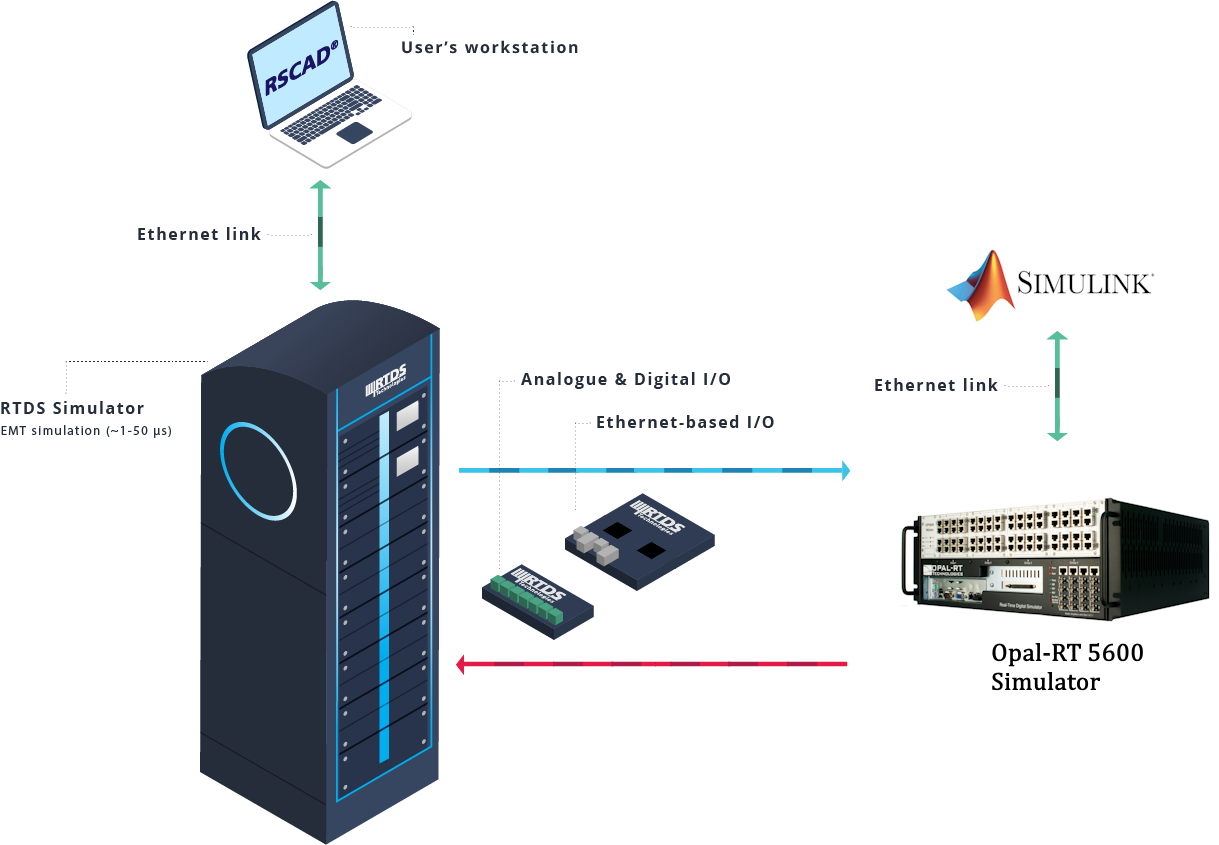
\includegraphics[width = 1\columnwidth]{hil_bench.png}
    \caption{Hardware-in-the-loop test bench.}
    \label{fig:hil_bench}
\end{figure}


\section{Description of the Physical grid}\label{sec:ch4/sec1}

For the test case, the simplified microgrid structure with distributed energy resources depicted in Figure~\cref{fig:cs_microgrid} has been chosen. It consists of the feeder 0.4 $kV$ feeder with a nominal frequency of 50 $Hz$, connected to the distribution grid via a 6/0.4 kV power transformer. The microgrid includes three connected DERs throw 4Q power inverters working in grid following mode. In addition, three consumers are connected, represented by a flexible load with active and reactive power set-points. All elements in the grid are connected with transmission lines, which are basically RL elements.

\begin{figure}[ht]
    \centering
    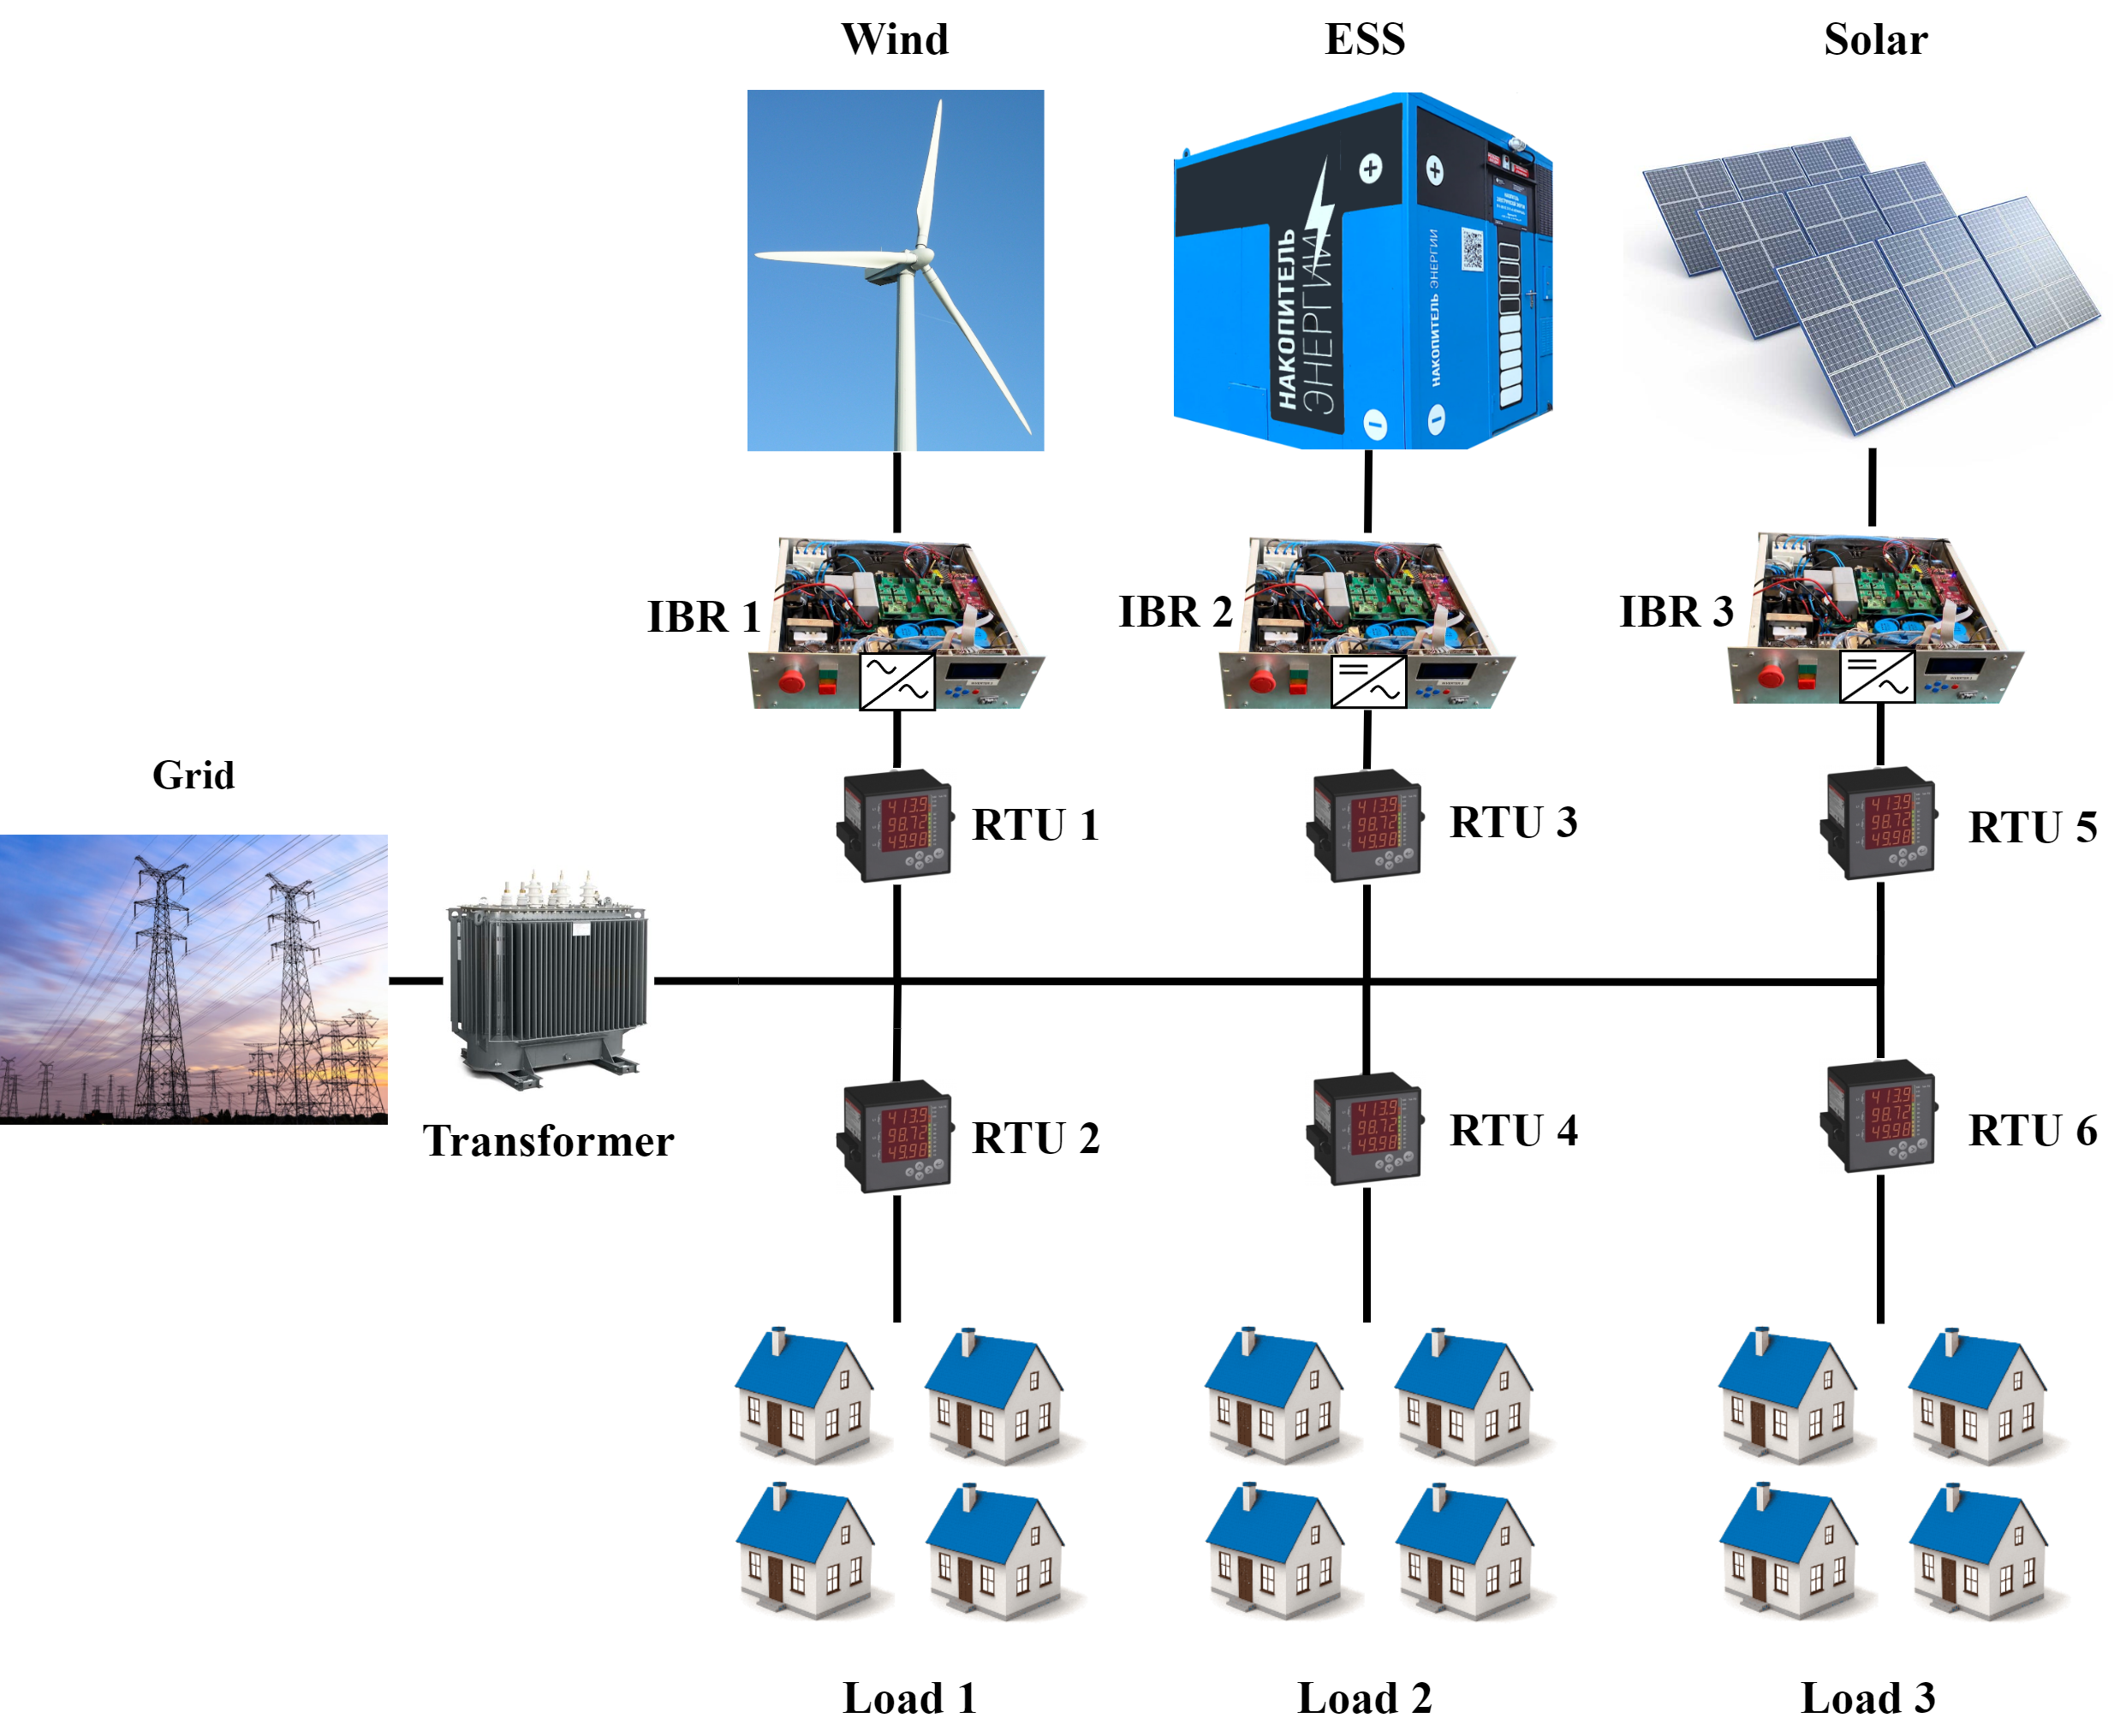
\includegraphics[width = 1\columnwidth]{cs_microgrid.png}
    \caption{Simplified microgrid structure with distributed energy resources.}
    \label{fig:cs_microgrid}
\end{figure}

According to the definition of DT technology in Section \ref{sec:dt_approach}, we must have a physical object with which to test the DT approach. HIL test bench allows us to realize the physical object as real hardware-connected throw amplifier or fully detailed EMT models. The basic parameters of the EMT model follow Table \ref{tab:base_model_param}.  The renewable generation and storage system are in the center of interest of this work and will be further discussed in detail. 


\begin{table}[htbp]
\centering
    \caption{RTDS EMT Model Parameters}
\begin{tblr}{
  hlines,
  vlines,
}
\textbf{Parameter} & \textbf{Quantity} & \textbf{Value} \\
    $T_{s}$ & Main model execution time  & 50 $us$    \\
    % $t_{\delta}$ &  Data exchange delay  & 10 ms \\
    $V_{g}$ & Grid nominal voltage  & 0.4 $kV$    \\
    $V_{g}$ & Grid nominal frequency   & 50 $Hz$   \\
    $P_{n}$ & Load/Generators nominal power   & 100 $kVA$   \\
    $TL_{R}$ &  TL active resistance  & 0.01644 $Ohm/km$ \\
    $TL_{L}$ &  TL reactive resistance  & 0.003048 $Ohm/km$ \\
    % $TL_{R}, TL_{L}$ &  {TL active resistance and\\ reactive resistance}  & {0.01644 $Ohm/km$,\\ 0.003048 $Ohm/km$} \\
\end{tblr}
\label{tab:base_model_param}
\end{table}

\subsection{Photovoltaics}\label{subsec:ch4/sec1/sub1}
Solar generation is presented by EMT blocks from the RTDS software library. The RTDS photovoltaic model consists of an array of solar cells, a mathematical model of which is represented as a current source in parallel with a single diode, as shown in Figure~\cref{fig:pv_model}. 

\begin{figure}[ht]
    \centering
    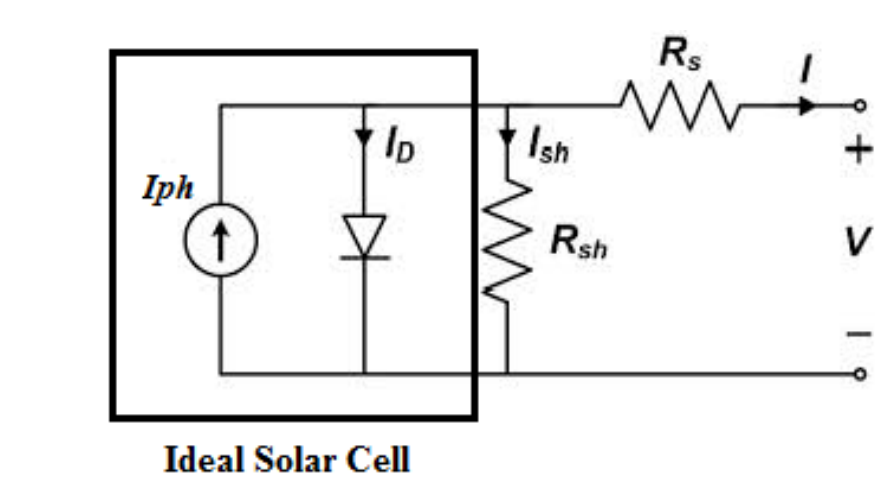
\includegraphics[width = 0.7\columnwidth]{pv_model.png}
    \caption{Equivalent model of solar cell in RTDS simulator}
    \label{fig:pv_model}
\end{figure}

The parameters of the solar cell are presented in Table \ref{tab:pv_model_param}. The number of modules is selected in such a way as not to exceed the common voltage of 700 $V$ on the DC bus and around 100 $kW$ at the maximum power point. The temperature regime chosen as normal and suggested as a constant of 25 degrees. The solar intensity input follows the profile with setpoints, the form of which is typical for the south of Russia. 

\begin{table}[htbp]
\centering
    \caption{Photovoltaics Module Parameters}
\begin{tblr}{
  hlines,
  vlines,
}
\textbf{Name} & \textbf{Description} & \textbf{Value} \\
    $N_c$ & {Number of series connected cells\\ per string per module} & 40 \\
    $N_{cp}$ & Number of parallel strings of cells & 10 \\
    $V_{ocref}$ & Open circuit voltage & 21.7 $V$\\ 
    $I_{scref}$ & Short circuit current & 3.35 $A$\\
    $V_{mpref}$ & Voltage at Pmax  & 17.4 $V$\\
    $I_{mpref}$ & Current at Pmax  & 3.05 $A$\\
    $E_g$ & {Energy gap: select semiconductor\\ material of solar cell} & {Monocrystalline\\ Silicon} \\
    $J_{tmp}$ & Short circuit current temperature coefficient & 0.065 $\%/^\circ C$\\
    $K_v$ & Open circuit voltage temperature coefficient & -0.56 $\%/^\circ C$\\
    $T_{ref}$ & Reference temperature at standard test conditions & 25 $^\circ C$\\
    $INS_{ref}$ & Initial reference solar intensity & 1000 $W/m^2$ \\
    $R_{so}$ & Open circuit series resistance & 0.5 $Ohm$\\
    $R_{sho}$ & Short circuit shunt resistance & 100 $Ohm$\\
\end{tblr}
\label{tab:pv_model_param}
\end{table}

The solar module is connected to the grid throw IBR with an integrated maximum power point tracking mechanism. IBR involved as three-phase inverter with boost converter in series according the schematic in Figure~\cref{fig:pv_ibr}.
% , following the parameters in Table \ref{tab:pv_ibr_param}. 

\begin{figure}[ht]
    \centering
    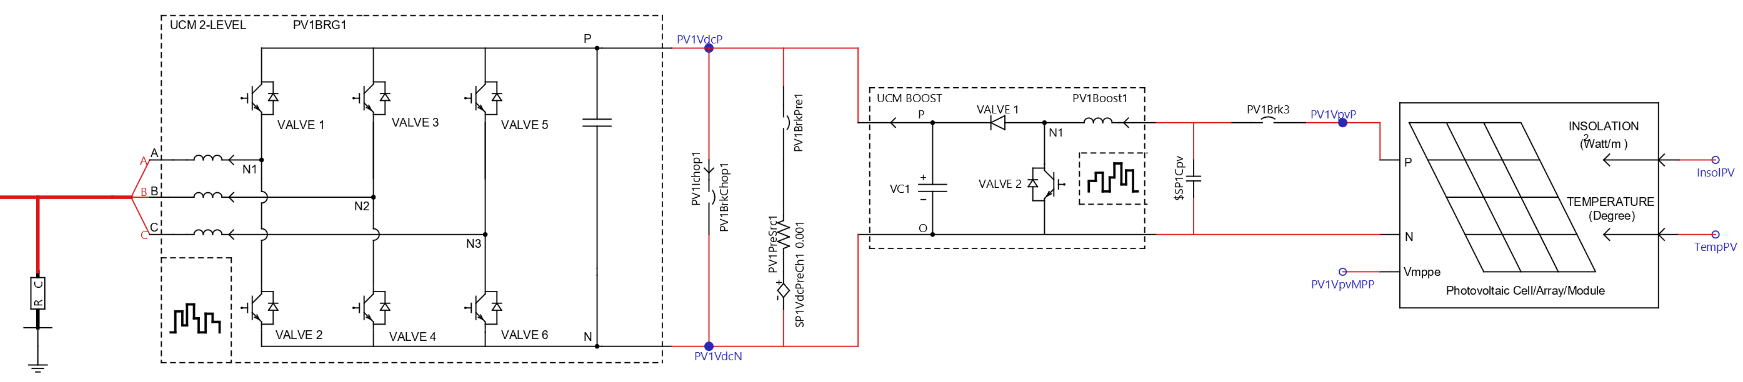
\includegraphics[width = 1\columnwidth]{pv_ibr.png}
    \caption{Photovoltaic array module with IBR connection}
    \label{fig:pv_ibr}
\end{figure}

% \begin{table}[h]
% \centering
%     \caption{EMT Model Parameters for PV-to-Grid IBR Interface}
% \begin{tblr}{
%   hlines,
%   vlines,
% }
% {Parameter & Quantity & Value} \\
%     $P_{ibr}$ & IBR nominal power   & 100 kVA   \\
%     $F_{sw}$ & IBR PWM base frequency  & 20 kHz    \\
%     $L_{1}, L_{2}$  & IBR Filter inductance  & {6.2 mH,\\ 4.58 uH}  \\ 
%     $R_{1}, R_{2}$  & IBR Filter resistance  & {19.6 mOhm,\\ 0.14 uOhm}  \\ 
%     $C_{f}$  & IBR Filter capacitance  & 82.89 uF   \\ 
%     $K_{p}^{cc}$ & {IBR Current control\\ proportional gain}  & 9.36   \\
%     $K_{i}^{cc}$ &  IBR Current control integral gain  & 29.4   \\
%     $K_{p}^{pll}$ &  IBR PLL proportional gain  & 5   \\
%     $K_{i}^{pll}$ &  IBR PLL integral gain  & 0,1 
% \end{tblr}
% \label{tab:pv_ibr_param}
% \end{table}

\subsection{Wind turbine}\label{subsec:ch4/sec1/sub2}

The wind turbine model represented by the dynamic model of a Type 4 wind power generator, the scheme of which is depicted in Figure~\cref{fig:wt_scheme}. The standard RTDS model is based on a variable-speed wind turbine with Permanent Magnet Synchronous Machine (PMSM) and connected to an AC grid through a full-scale back-to-back three-level VSC. The time domain modeling of this PMSM model is based on the theory $dq0$. The $dq$ equivalent circuit of the PMSM is shown below in Figure~\cref{fig:pmsm_model}. 

\begin{figure}[ht]
    \centering
    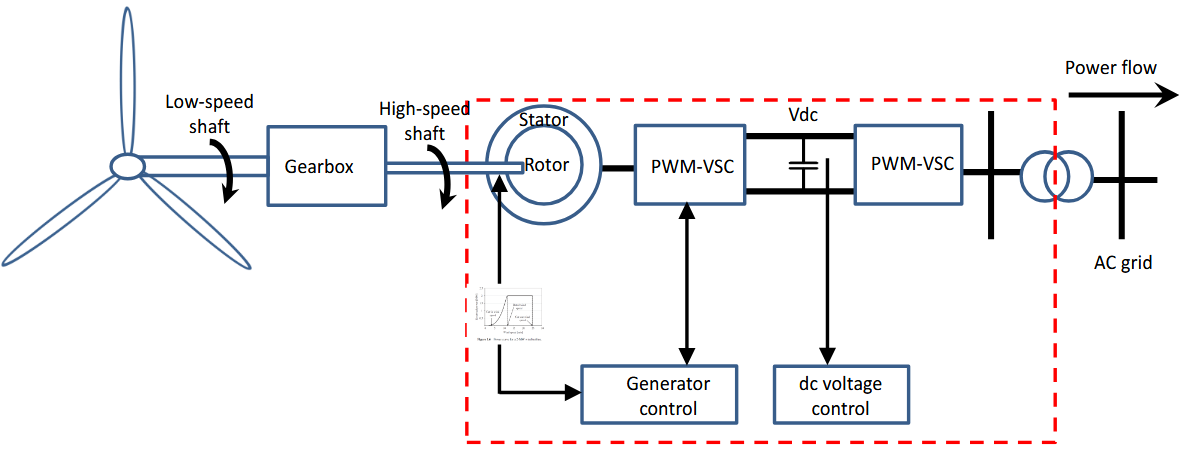
\includegraphics[width = 1\columnwidth]{wt_scheme.png}
    \caption{Schematic block diagram of type 4 wind generation model in RTDS simulator}
    \label{fig:wt_scheme}
\end{figure}
\begin{figure}[ht]
    \centering
    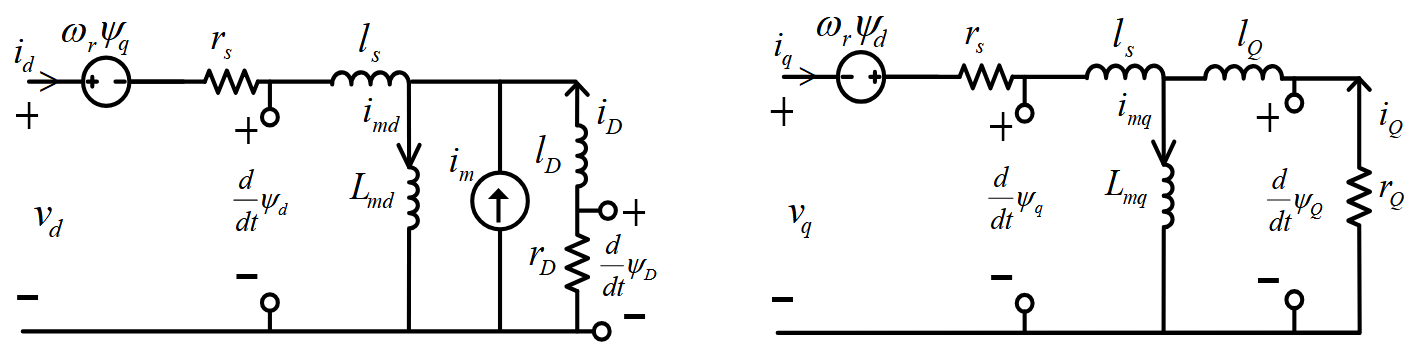
\includegraphics[width = 1\columnwidth]{pmsm_model.png}
    \caption{Equivalent PMSM Model in RTDS simulator}
    \label{fig:pmsm_model}
\end{figure}

The VSC simulated by detailed EMT model with 12 power transistors, which is AC/DC and DC/AC parts in series, firing by PWM plant. The DC/AC part follows the same parameter as for solar IBR from Table \ref{tab:pv_ibr_param}. The output power limited by 100 $kW$ and the reference set point follow the profile characteristic for the south regions of Russia. As models consist of many blocks with complex control systems, the only most sensitive parameters are presented in Table \ref{tab:wt_model_param}. 

\begin{table}[htbp]
\centering
    \caption{RTDS EMT Wind Turbine Model Parameters}
\begin{tblr}{
  hlines,
  vlines,
}
\textbf{Name} & \textbf{Description} & \textbf{Value} \\
    % $V_r$ & {Rated Voltage (L-L RMS)} & 0.690 $kV$ \\
    $P_{n}$ & Rated MVA of the Machine & 0.1 $MVA$ \\
    $X_s$ & Stator Leakage Reactance & 0.1 $pu$\\ 
    $X_{md}$ & D-axis Unsaturated Magnet Reactance & 0.5 $pu$\\
    $X_D$ & D-axis Damper Leakage Reactance  & 2.265 $pu$\\
    $X_{mq}$ & Q-axis Magnetizing Reactance  & 0.2 $pu$\\
    $X_Q$ & Q-axis Damper Leakage Reactance & 2.265 $pu$ \\
    $r_s$ & Stator Resistance & 0.01 $pu$\\
    $r_D$ & D-axis Damper Resistance & 2.0 $pu$\\
    $r_Q$ & Q-axis Damper Resistance & 2.0 $pu$\\
    $V_{dc}$ & Rated DC voltage (pole-pole) & 1.2 $kV$\\
    $R_{dc}$ & DC link R & 0.1 $m\Omega$\\
    $L_{dc}$ & DC link L & 2 $\mu H$\\
    $C_{dc}$ & Aggregated Smoothing capacitor (C/2) & 2000 $mF$\\
    $F_{sw}^{pmsm}$ & Switching Frequency (PMSM-side converter)  & 3 $kHz$\\
    $F_{sw}^{ac}$ & Switching Frequency (Grid-side converter)  & 20 $kHz$
\end{tblr}
\label{tab:wt_model_param}
\end{table}


\subsection{Energy Storage System}\label{subsec:ch4/sec1/sub3}

Dynamic Digital Mirroring applicable for all participant of energy exchange and ESS a powerful example of it, and a vivid example of it is a  VRFBs. The VRFB (5 kW/ 10 kWh) at the Skolkovo Institute of Science and Technology, that shown in Figure~\cref{fig:vrfb_setup},  was elaborated to gather experimental data. The parameters of the system are listed in Table \ref{tab:vrfb_setup_param}.

\begin{figure}[ht]
    \centerfloat{
        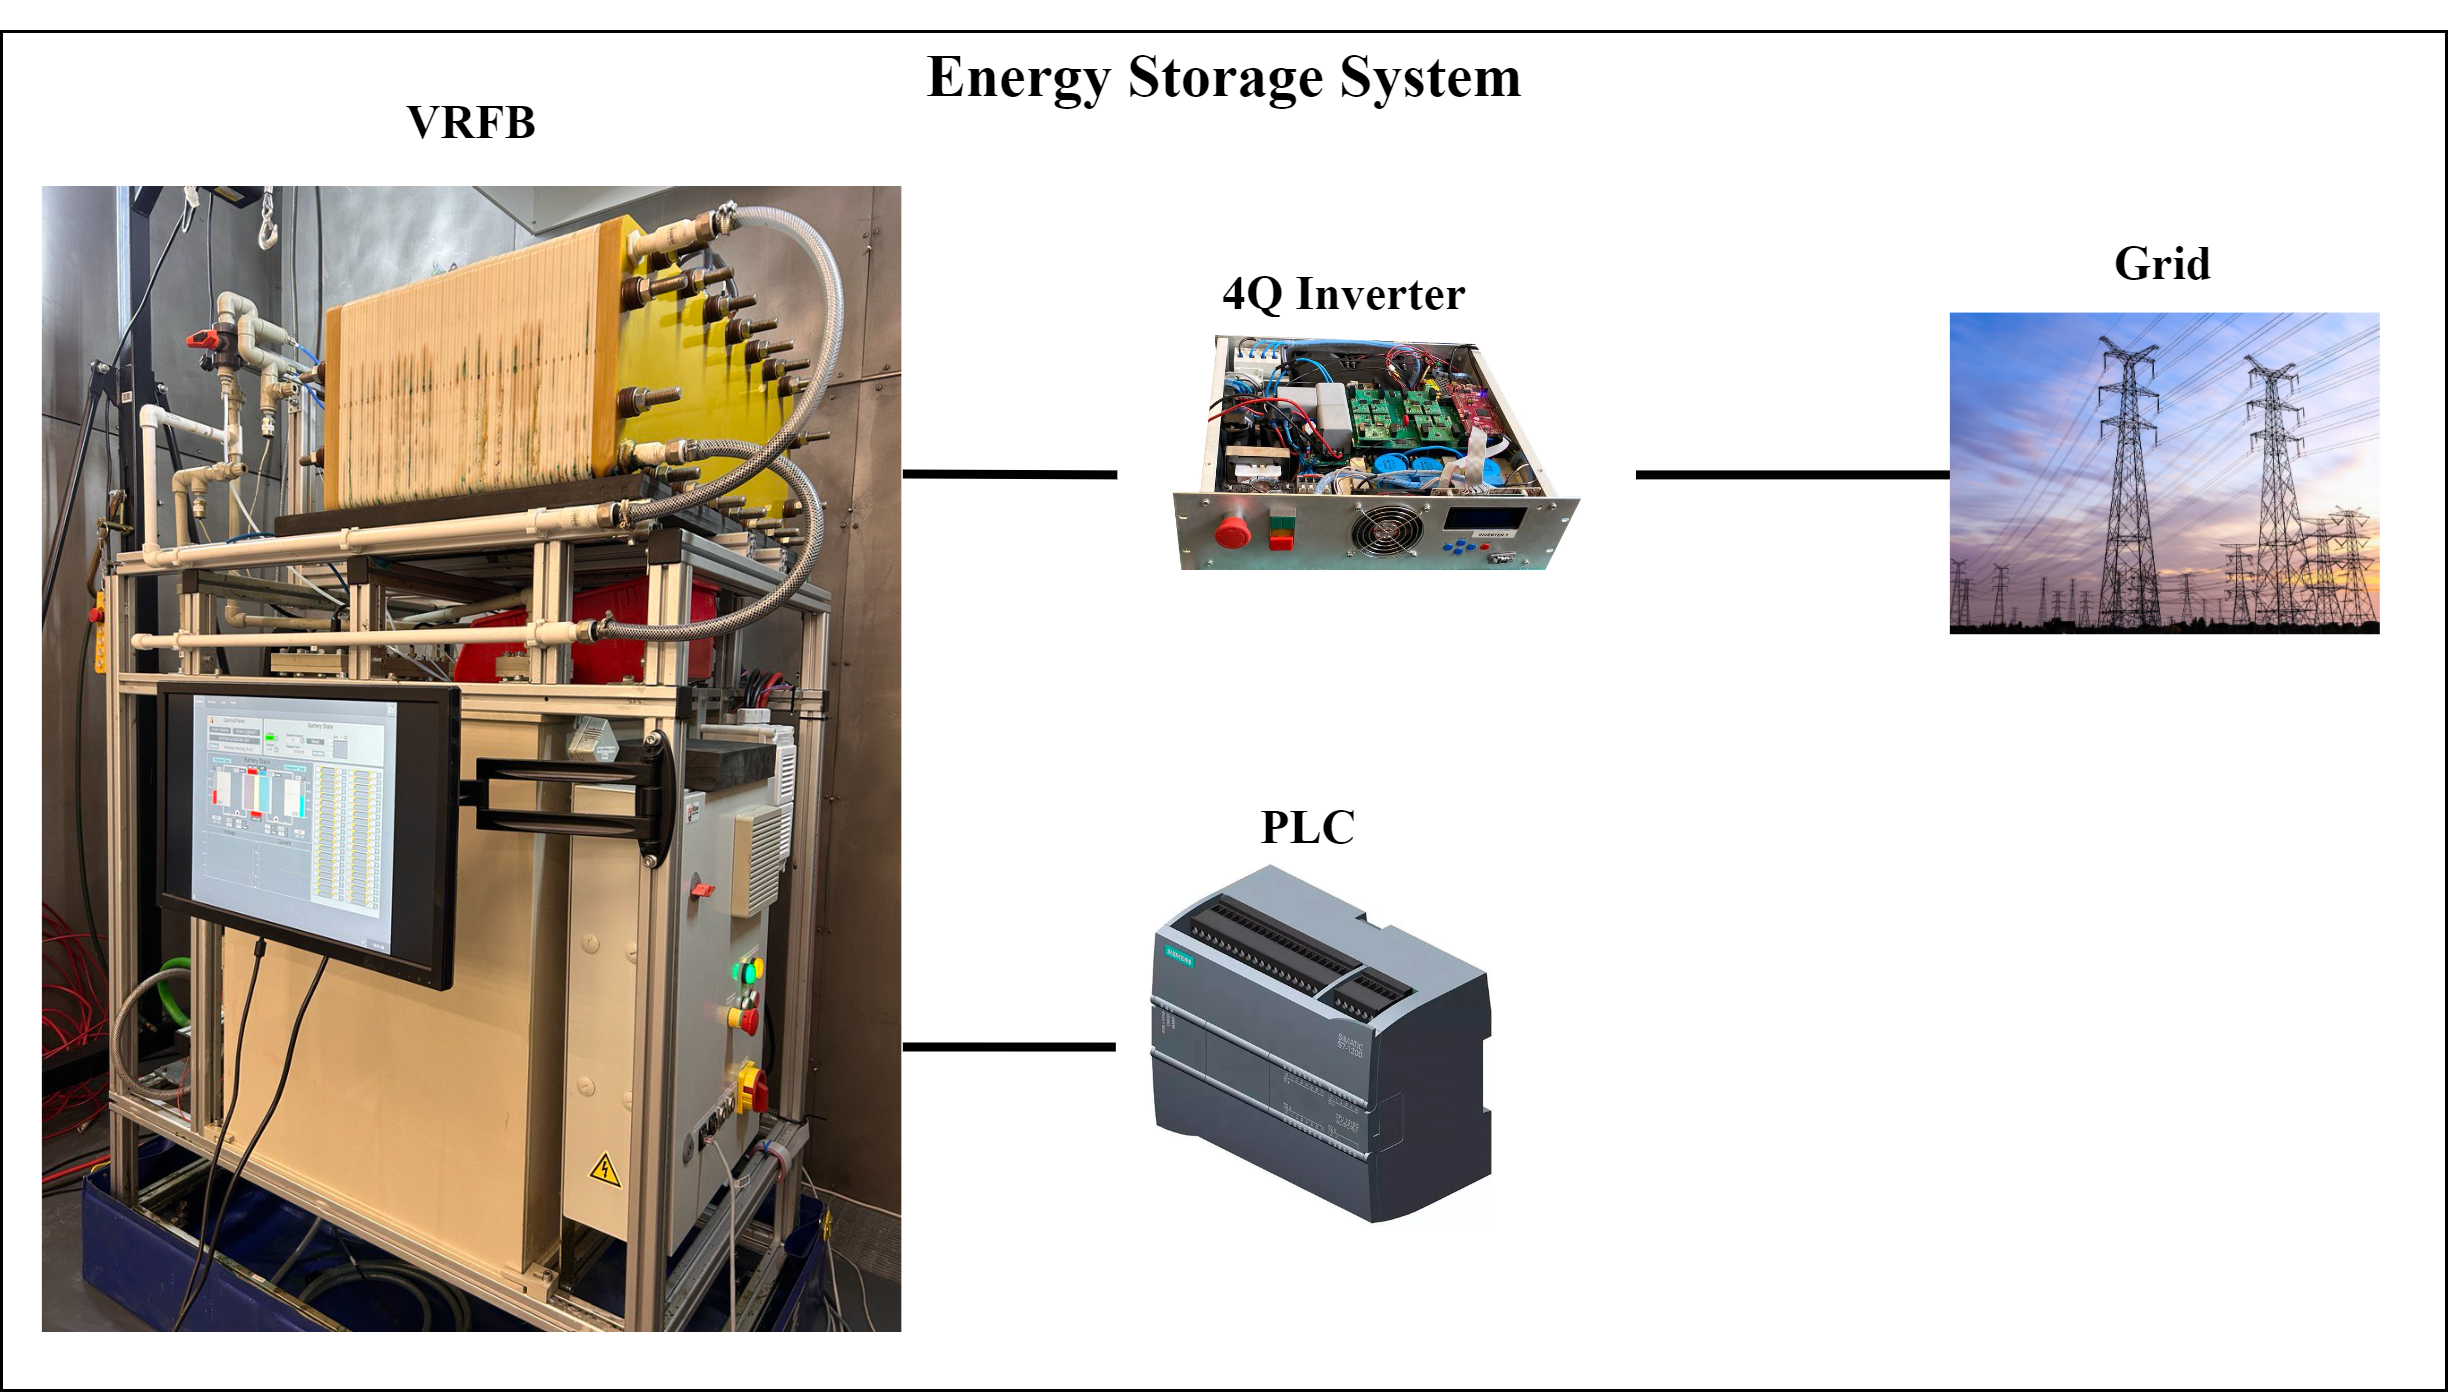
\includegraphics[scale=0.8]{vrfb_setup.png}
    }
    \caption{The VRFB (5 kW/ 10 kWh) setup.}\label{fig:vrfb_setup}
\end{figure}

\begin{table}[htbp]
\centering
    \caption{Specification of VRFB Experimental Setup}
\begin{tblr}{
  hlines,
  vlines,
}
\textbf{Name} & \textbf{Description} & \textbf{Value} \\
    $V_{tk}$ & Electrolyte volume held in the storage tanks & 0.045 $m^3$ \\
    $L \times h \times w$ & Electrode's geometrical dimensions & $325 \times 190 \times 3$ $mm$ \\
    $V_{cell}$ & Half-cell's electrolyte content volume & $27 \cdot 10^{-5}$ $m^3$\\ 
    $A_m$ & Membrane area & 0.0848 $m^2$\\
    $N$ & Number of cells in the stack  & 38 \\
    $d_m$ & Membrane thickness,  & $5 \cdot 10^{-5}$ $m$\\
    $c_b$ & Baseline levels of vanadium ions present & 1106 $mol ~m^{-3}$ \\
    $Q$ & Range of flow rates & $[4 ; 10]$ $l ~min^{-1}$\\
    $V_{cut}$ & Cut-off voltages & $[40 ; 65]$ $V$\\
    $SOC_{\Delta}$ & Operating SoC range & $[5 ; 95]$ $\%$\\
    $I_{\Delta}$ & Applied current range & $[0 ; 60]$ $A$\\
    - & Membrane type & AEM\\
    $I_{\Delta}$ & Applied current range & $[0 ; 60]$ $A$\\
\end{tblr}
\label{tab:vrfb_setup_param}
\end{table}

Applying the identification method from Section \ref{subsec:ch3/sec1/sub1} the equivalent overall vanadium concentration $c_b$, the crossover multiplication factor $\gamma$, the formal potential of the cell $U_0^*$, cell resistivity $r_{c e l l}$, the slope $\alpha$ and the growth rate  $\beta$ of the mass transfer coefficient were estimated and presented in Table \ref{tab:vrfb_idtf_param}. 

\begin{table}[htbp]
\centering
    \caption{Identified parameters of VRFB Experimental Setup}
\begin{tblr}{
  hlines,
  vlines,
}
\textbf{Name} & \textbf{Description} & \textbf{Value} \\
    $\gamma$ & Crossover factor & 1.03 $m^3$ \\
    $c_0$ & Equivalent overall  battery concentration & $1.450 \times 10^3$ $mol/m^{3}$ \\
    $ASR$ & Area specific resistance & 2.231 $\Omega cm^2$\\ 
    $U_0^*$ & Formal potential & 1.38 $V$\\
    $\alpha$ & Slope of mass transfer  coefficient  & $1.64 \times 10^{-4}$ \\
    $\beta$ & Growth of mass transfer  coefficient  & 0.4\\
\end{tblr}
\label{tab:vrfb_idtf_param}
\end{table}


% These relates with internal physical and chemical processes that occur during operation, such as the undesired migration of vanadium ions via the membrane, electrode activation, concentration, and ohmic polarizations, as well as capacity deterioration over time because of uneven vanadium concentrations. For identification of the VRFB system parameters we used the approach proposed in our previous work \cite{jrn_bogdanov_2023}.

% The VRFB model presented above involves the identification of six unknown parameters, including the equivalent overall vanadium concentration $c_b$, the crossover multiplication factor $\gamma$, the formal potential of the cell $U_0^*$, cell resistivity $r_{c e l l}$, the slope $\alpha$ and the growth rate  $\beta$ of the mass transfer coefficient:
% \begin{equation}
%     \label{eq:idn}
%     \xi=\left(c_b, \gamma, r_{c e l l}, U_0^*, \alpha, \beta\right)^T .
% \end{equation}

% To be as close as possible to real conditions, the VRFB (5 kW/ 10 kWh) at the Skolkovo Institute of Science and Technology was used with Ponovo amplifier as interface to HIL simulator, as shown in Figure~\cref{fig:vrfb_panovo}. The parameters of the system are listed in Table \ref{tab:vrfb_setup_param}.

% \begin{figure}[htbp]
%     \centering
%     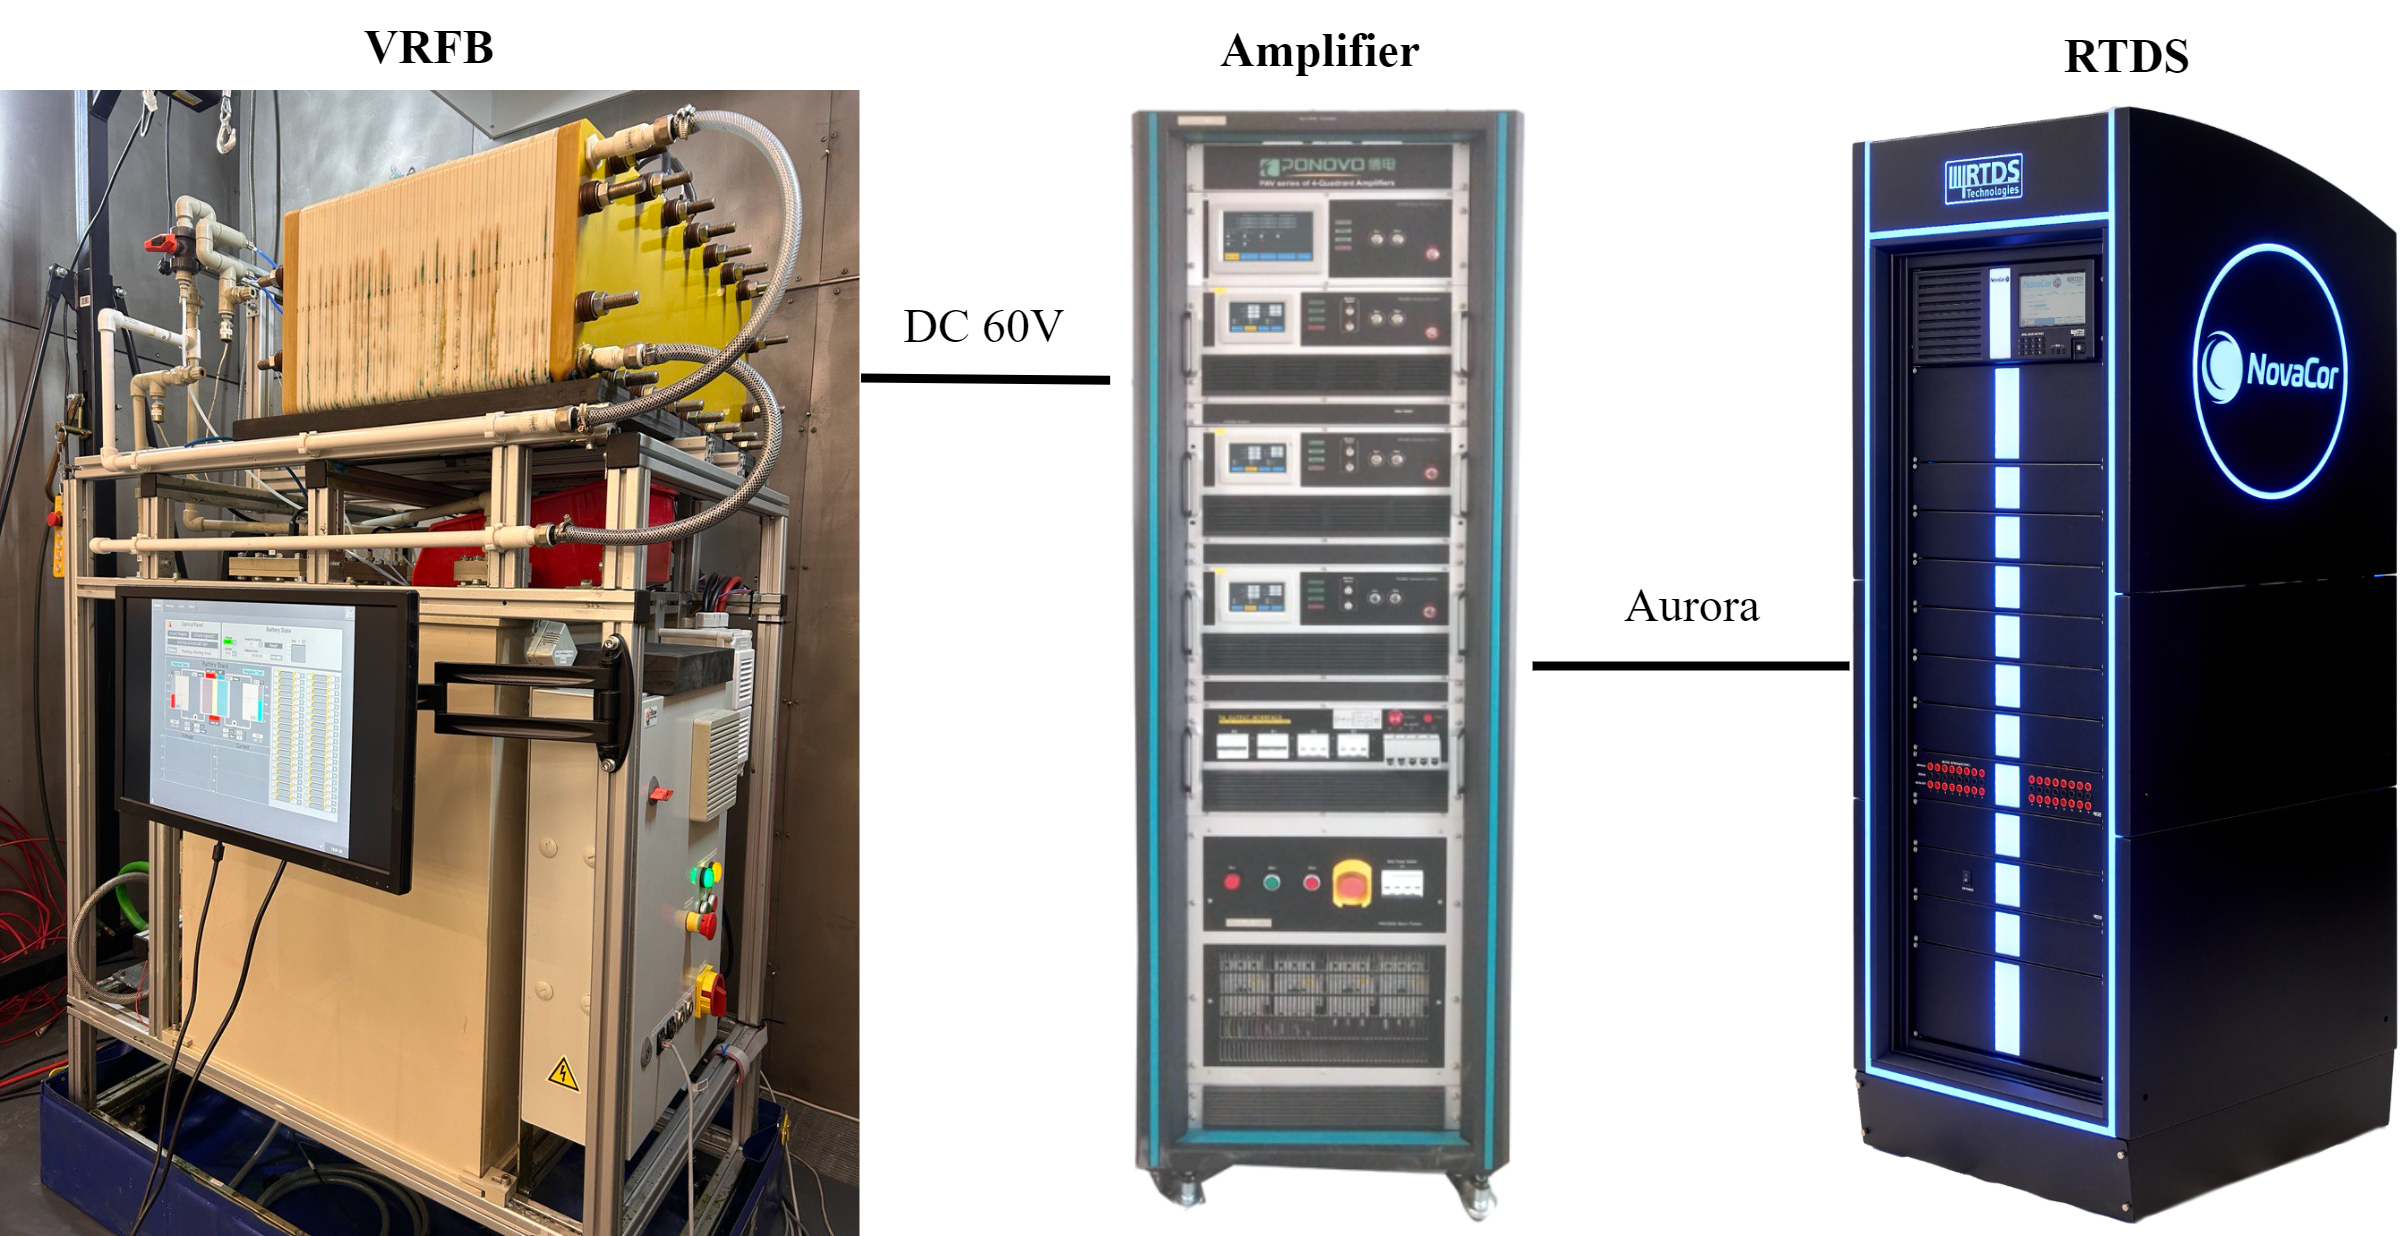
\includegraphics[width = 1\columnwidth]{vrfb_panovo.png}
%     \caption{Equivalent PMSM Model in RTDS simulator}
%     \label{fig:vrfb_panovo}
% \end{figure}

% The ultimate design of the DT for the VRFB state of charge estimator is depicted in Fig.~\ref{fig:vrfb_dt}. By leveraging digital twin technology, this state estimator acquires and interprets signals related to current, temperature, and flowrate, achieving real-time dynamic monitoring of the battery's state, SOC and output stack voltage particularly. 


The system is equipped with industrial-grade sensors such as ambient temperature, open-circuit voltage at stack input, flow rate of positive electrolyte, flow rate of negative electrolyte, output stack voltage and current. Sensor measurements collected by PLC, which are then transmitted to an OPC server via Modbus TCP protocol.

\section{Description of the Digital Twin}\label{sec:ch4/sec2}

The ultimate design of the DT for the VRFB dynamic mirroring is depicted in Figure~\cref{fig:vrfb_dt}. By leveraging digital twin technology, this estimator acquires and interprets signals related to current, temperature, and flowrate, achieving real-time monitoring of the battery's state. This setup provides accurate SOC and output stack voltage, tacking into accoun degradation of battery and crossover effect \autocite{10615087}.

\begin{figure}[htbp]
    \centerfloat{
        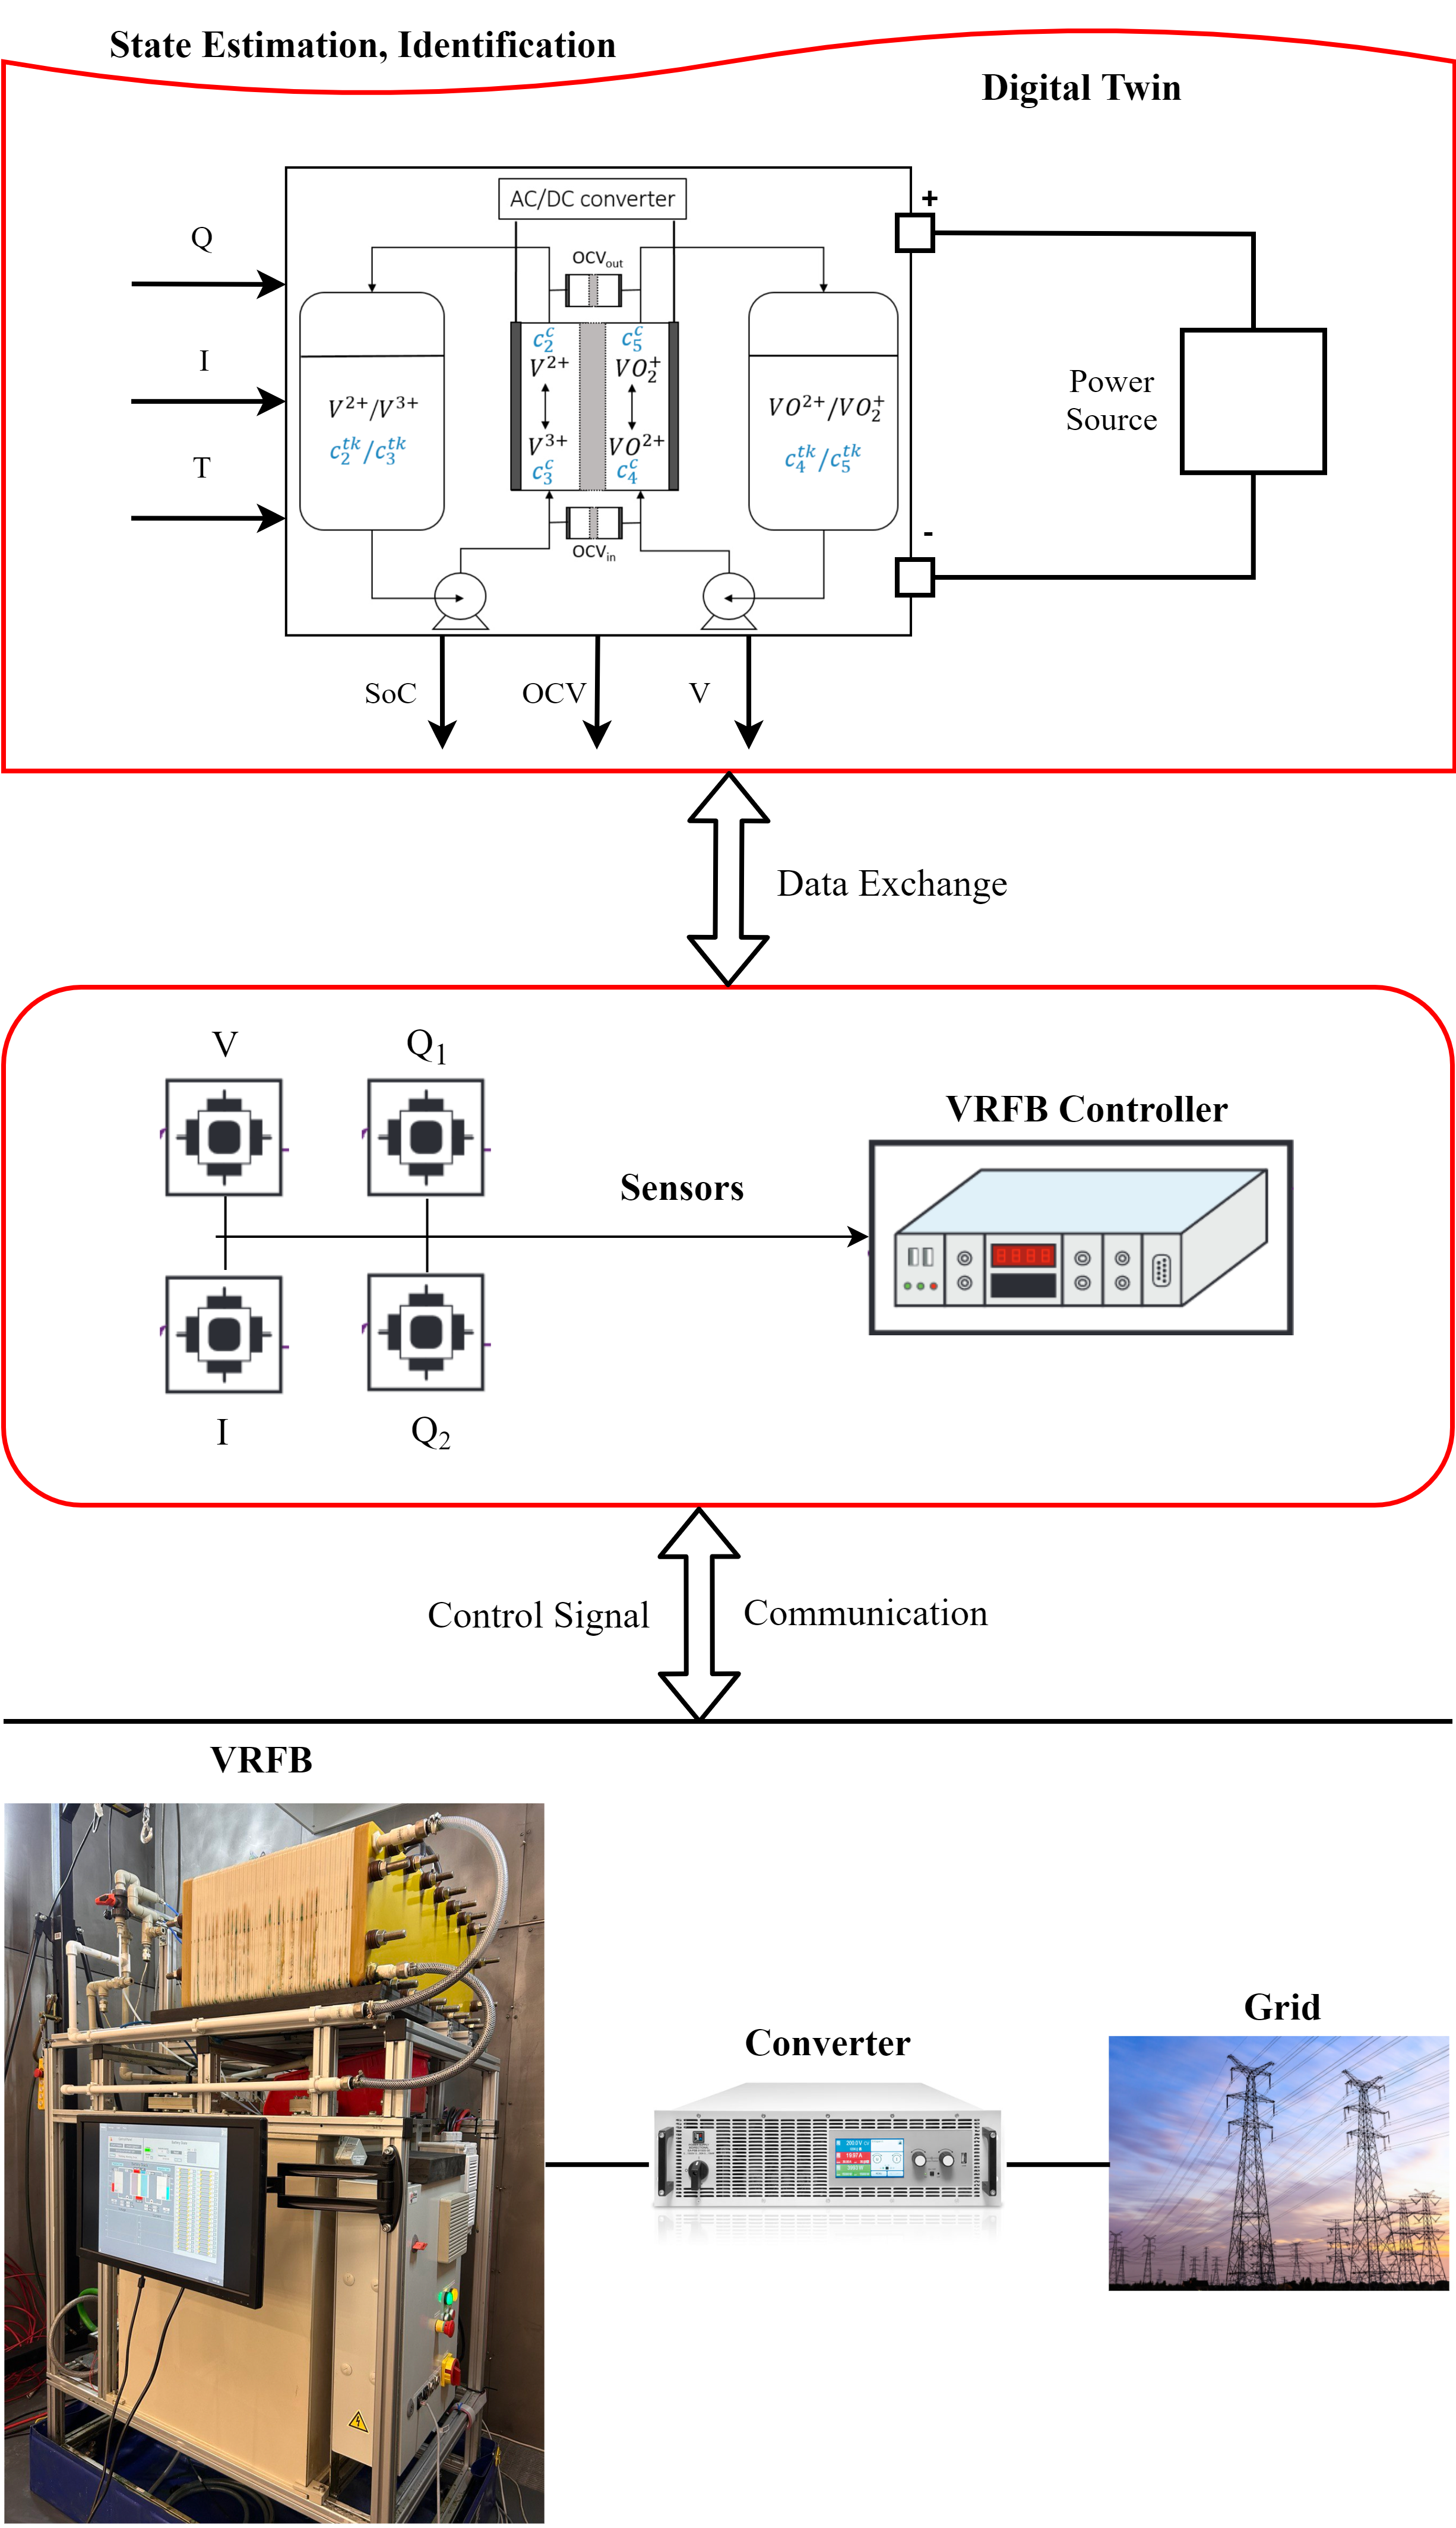
\includegraphics[scale=0.9]{vrfb_dt}
    }
    \caption{Flowchart of the DT based SoC estimation.}\label{fig:vrfb_dt}
\end{figure}

To mirror the dynamic picture of the whole feeder, the DT dynamic model must be consisted of the aggregated discrete inverter model working in grid-following mode and receiving power references from measurements devices installed in physical grids in PCC. According to the DT building method described in Chapter \ref{ch:ch3}, the aggregated discrete inverter model can be implemented with connection to the grid network consisting of RL equivalents of transmission lines. At first, the inverter parameters must be obtained for grid-following mode. 

Basically, we can find ourselves in three different situations. All inverter parameters are known from the beginning of the DT building process, and the connected generator represents to us as a white box. This situation is more specific for the transmission grid level which is strongly regulated and all generative equipment is checking for compatibility. For low voltage level, distribution grid, which we assumed to test, the connected equipment is presented by hundreds of suppliers and parameters usually hidden for us. In this case, the connected generator is represented as a black box. 

As a possible way to deal with that is to try to move in gray box section where parameters are partially available. It can be reached by taking into account that information about the maximum power level is usually available. For example, the typical household connection in Russia is limited to 15 $kW$. The renewables from small commercial owners does not exceed hundreds of kW and is also agreed prior to the permit being issued. Another suggestion may be that the usual PWM frequency accepted in industry is 20 or 40 kHz. Thus, the initial parameters for calculating the filter components are as follows.

\begin{table}[htbp]
\centering
    \caption{Initial Electrical Parameters of the Inverter}
\begin{tblr}{
  hlines,
  vlines,
}
\textbf{Name} & \textbf{Description} & \textbf{Value} \\
    $V_{n}$ & Grid voltage & 230 $V$ \\
    $P_{n}$ & Output power of the inverter & 100 $kVA$ \\
    $V_{dc}$ & DC-Link voltage & 700 $V$\\ 
    $F_g$ & Grid frequency & 50 $Hz$\\
    $F_{sw}$ & Switching frequency  & 20 $kHz$ \\
    $PF$ & Power factor  & 1 \\
\end{tblr}
\label{tab:ibr_initial_param}
\end{table}

Following the well-known LCL filter design for grid-connected system \autocite{Kahlane2015LCLFD}, we calculate at the beginning the base impedance and capacitance, respectively: 
\begin{equation}
    \begin{aligned}
        & \mathrm{Z}_{\mathrm{b}}=\mathrm{U}_{\mathrm{n}}^{2} / \mathrm{S}_{\mathrm{n}} = 0.529,\\
        & \mathrm{C}_{\mathrm{b}}=1 / \omega_{\mathrm{n}} \times \mathrm{Z}_{\mathrm{b}} = 0.006.
    \end{aligned}
\end{equation}

Inverter side inductance $L_i$ allows to limit the output current ripple by up to 10\% of the nominal amplitude.
\begin{equation}
    \begin{aligned}
        & \Delta \mathrm{I}_{\mathrm{L}-\max }=0.01 \frac{\mathrm{P}_{\mathrm{n}} \sqrt{2}}{\mathrm{V}_{\mathrm{n}}} = 6.15,\\
        & \mathrm{L}_{\mathrm{inv}}=\frac{\mathrm{U}_{\mathrm{DC}}}{16 \mathrm{F}_{\mathrm{sw}} \Delta \mathrm{I}_{\mathrm{L}-\max }} = 3.56e-04.
    \end{aligned}
\end{equation}

The filter capacity based on the maximal power factor variation acceptable by the grid is 5\% can be calculated as a multiplication of the system base capacitance $C_b$. The grid side inductance $L_g$ can be calculated based on the factor $r = 0.6$, between $L_{inv}$ and $L_g$:
\begin{equation}
    \begin{aligned}
        & C_{f}=0.05 C_{b} = 3e-04,\\
        & L_g = r \times L_{inv} = 2.14e-04.
    \end{aligned}
\end{equation}

The final phase of the design involves managing the filter's resonant frequency. It should be distinct from the grid frequency and at least half of the converter's switching frequency to ensure sufficient attenuation. The resonant frequency for the L-C-L filter is calculated by:
\begin{equation}
    \mathrm{w}_{\mathrm{res}}=\sqrt{\frac{\mathrm{L}_{\mathrm{inv}}+\mathrm{L}_{\mathrm{g}}}{\mathrm{~L}_{\mathrm{inv}} \times \mathrm{L}_{\mathrm{g}} \times \mathrm{C}_{\mathrm{f}}}} = 5e+03.
\end{equation}

In order to reduce oscillations and unstable states of the filter, the damping resistor is required:
\begin{equation}
    \mathrm{R}_{\mathrm{d}}=\frac{1}{3 \omega_{\mathrm{res}} \mathrm{C}_{\mathrm{f}}} = 0.256.
\end{equation}

The next step is to define the current control dynamics by defining the PI parameters based on (\ref{eq:cc_pi}). Suggesting recommended bandwidth of 1500 $rad/s$ for the current controller:
\begin{equation}
    \begin{array}{l}
        k_{p}=(L_{inv}+L_{g}) w_c = 0.854, \\
        k_{i}=\left(R_{inv}+R_{g}\right) w_c = 2.682.
    \end{array}
    \label{eq:cc_pi_num}
\end{equation}

The PLL parameters are not hidden and are usually provided by signal processor developers \autocite{ti_sprabt3a}. Thus, the full set of parameters involved in the dynamic modeling of inverters are summarized in Table \ref{tab:ibr_sum_param}.

\begin{table}[htbp]
\centering
    \caption{Summarized Parameters of Inverter Dynamic Model}
\begin{tblr}{
  hlines,
  vlines,
}
\textbf{Name} & \textbf{Description} & \textbf{Value} \\
    $L_{inv}$ & Inverter side inductance & 356 $\mu H$ \\
    $R_{inv}$ & Inverter side resistance & 1.1 $mOhm$ \\
    $L_{g}$ & Grid side inductance & 214 $\mu H$ \\
    $R_{g}$ & Grid side resistance & 67 $mOhm$ \\
    $C_{f}$ & Filter capacitance & 300 $\mu F$\\ 
    $R_d$ & Filter damping resistance & 256 $mOhm$\\
    $K_p^{cc}$ & Proportional part of current controller& 0.854 \\
    $K_i^{cc}$ & Integral part of current controller& 2.682 \\
    $K_p^{pll}$ & Proportional part of PLL controller& 5.0 \\
    $K_i^{pll}$ & Integral part of PLL controller& 0.1 \\    
\end{tblr}
\label{tab:ibr_sum_param}
\end{table}

Using the average dynamic modeling method with the parameters calculated above, three IBRs connected to transmission lines have been realized in the form of a discrete simulation model. The next step is to connect the model that represents the DT with the physical grid, using data exchange channels, according to the diagram, shown in Figure~\cref{fig:dt_dse}. 

\begin{figure}[htbp]
    \centering
    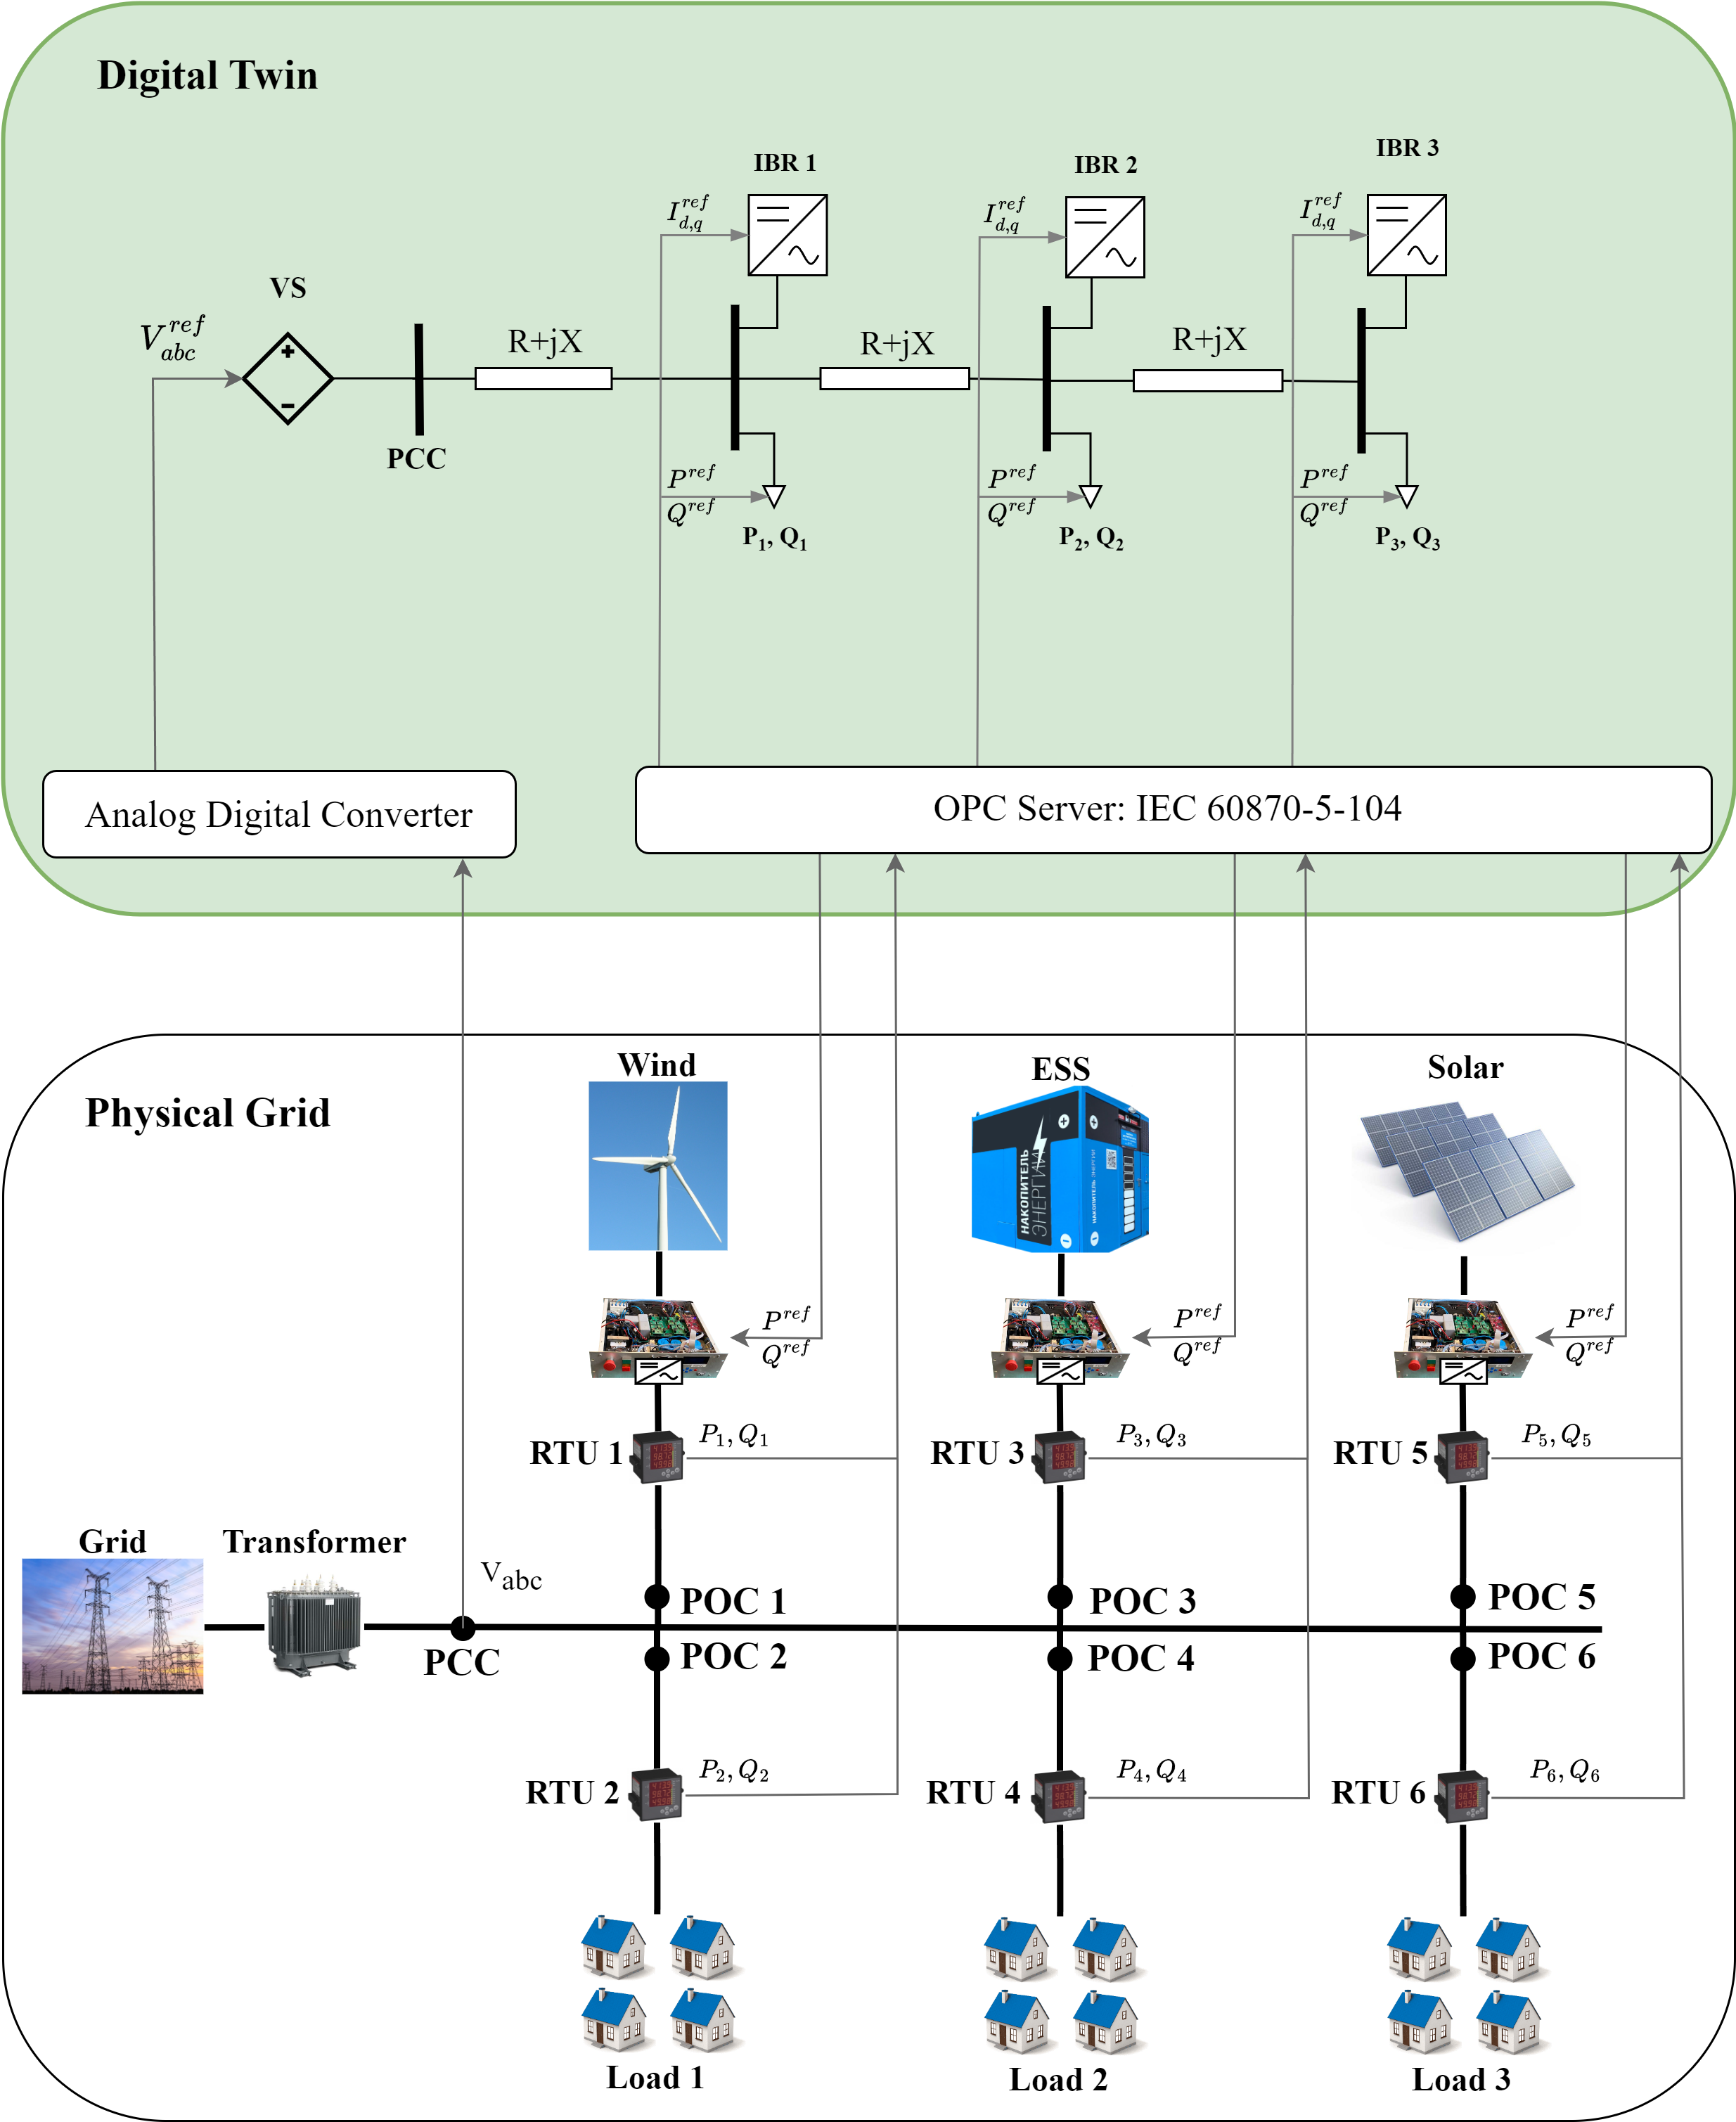
\includegraphics[width = 1\columnwidth]{dt_dse.png}
    \caption{Diagram of the DT based mirroring of PEDG.}
    \label{fig:dt_dse}
\end{figure}

Dynamic mirroring is achieved within computation devices that include analog/digital communication channels and where the DT real-time modeling is computed. The received three-phase voltage signal measured at the feeder head of the real grid is sent as a reference to the voltage source inside the virtual feeder in the DT model. It creates a reference sinusoidal voltage in the DT model, to which synchronizes all IBRs. The current flow in the virtual feeder is created by the power consumption of the virtual load and the bidirectional power flow of the virtual inverters. These allow real-time monitoring of the three-phase voltage and current sinusoidal signals at any location along the feeder.

\section{Digital Twin Transient Response Following}\label{sec:ch4/sec3}

\textbf{DT for VRFB validation}. To evaluate the DT model's ability to accurately respond to current variations, the power profiles for DC source were prepared and tested. At first, charging and discharging process were made with constant current mode according the profile in Figure~\cref{fig:statprofile_i} to identify the parameters of the battery. Figure~\cref{fig:statprofile_v} shows the voltage transients during power injection and consumption.

The Nernst equation's characterization of the open circuit voltage (OCV) is the most popular signal used in designing SOC observers of industrial scale batteries.  The Nernst law gives rise to the following equation, which can be employed to determine the SOC \cite{jrn_trovo_2020}:
\begin{equation}
    \label{eq:soc_ocv}
    S O C=\frac{e^{\left(O C V-U_0\right) n F / 2 R T}}{1+e^{\left(O C V-U_0\right) n F / 2 R T}}100,
\end{equation}
where $U_0 = 1.37 V$ is the formal potential for vanadium couples $(T = 298 K)$. 

Thus, there are two different methods that can be used for estimation of instant battery state of charge. The first approach is based on application of inlet OCV data following the indirect estimation of SOC with application of Nernst equation. The  second method is based on the direct calculation of the SOC from the concentrations of vanadium ions. Since the proposed DT methodology demonstrates the capacity to estimate the internal states by factoring in the vanadium species concentration, it enables us to calculate the SOC based on \cref{eq:soc_dt} and inlet OCV based on \cref{eq:ocv_dt}. 

\begin{equation}
    \label{eq:ocv_dt}
    OCV=U_0^*+\frac{R T}{F} \ln \left[\left(\frac{c_5}{c_4}\right)\left(\frac{c_2}{c_3}\right)\right].
\end{equation}

To show the high accuracy of this main indicators, an experiment was performed with multi-step constant current profile presented on Figure~\cref{fig:dynprofile_i}. The comparison of the inlet OCV curves and computed SOC based on different sources is shown in Figure~\cref{fig:dynprofile_ocv} and Figure~\cref{fig:dynprofile_soc} respectively. An additional feature of digital twin application is voltage monitoring, the result of which is shown in Figure~\cref{fig:dynprofile_v}.   

As can be seen from the plots, the battery behavior obtained by application of DT approach follows the VRFB test bench inlet OCV and stack output voltage measurements with high accuracy. It is allows to observe the SOC in real-time maintaining a maximum error below 3 \%.  

Notably, such accurate results can be achieved without the need for additional measurements, utilizing only flow rate, ambient temperature, and stack output current. These findings suggest the application of DT for online state estimation and filtering of corrupted data from sensors.

\begin{figure}[ht]
    \centerfloat{
        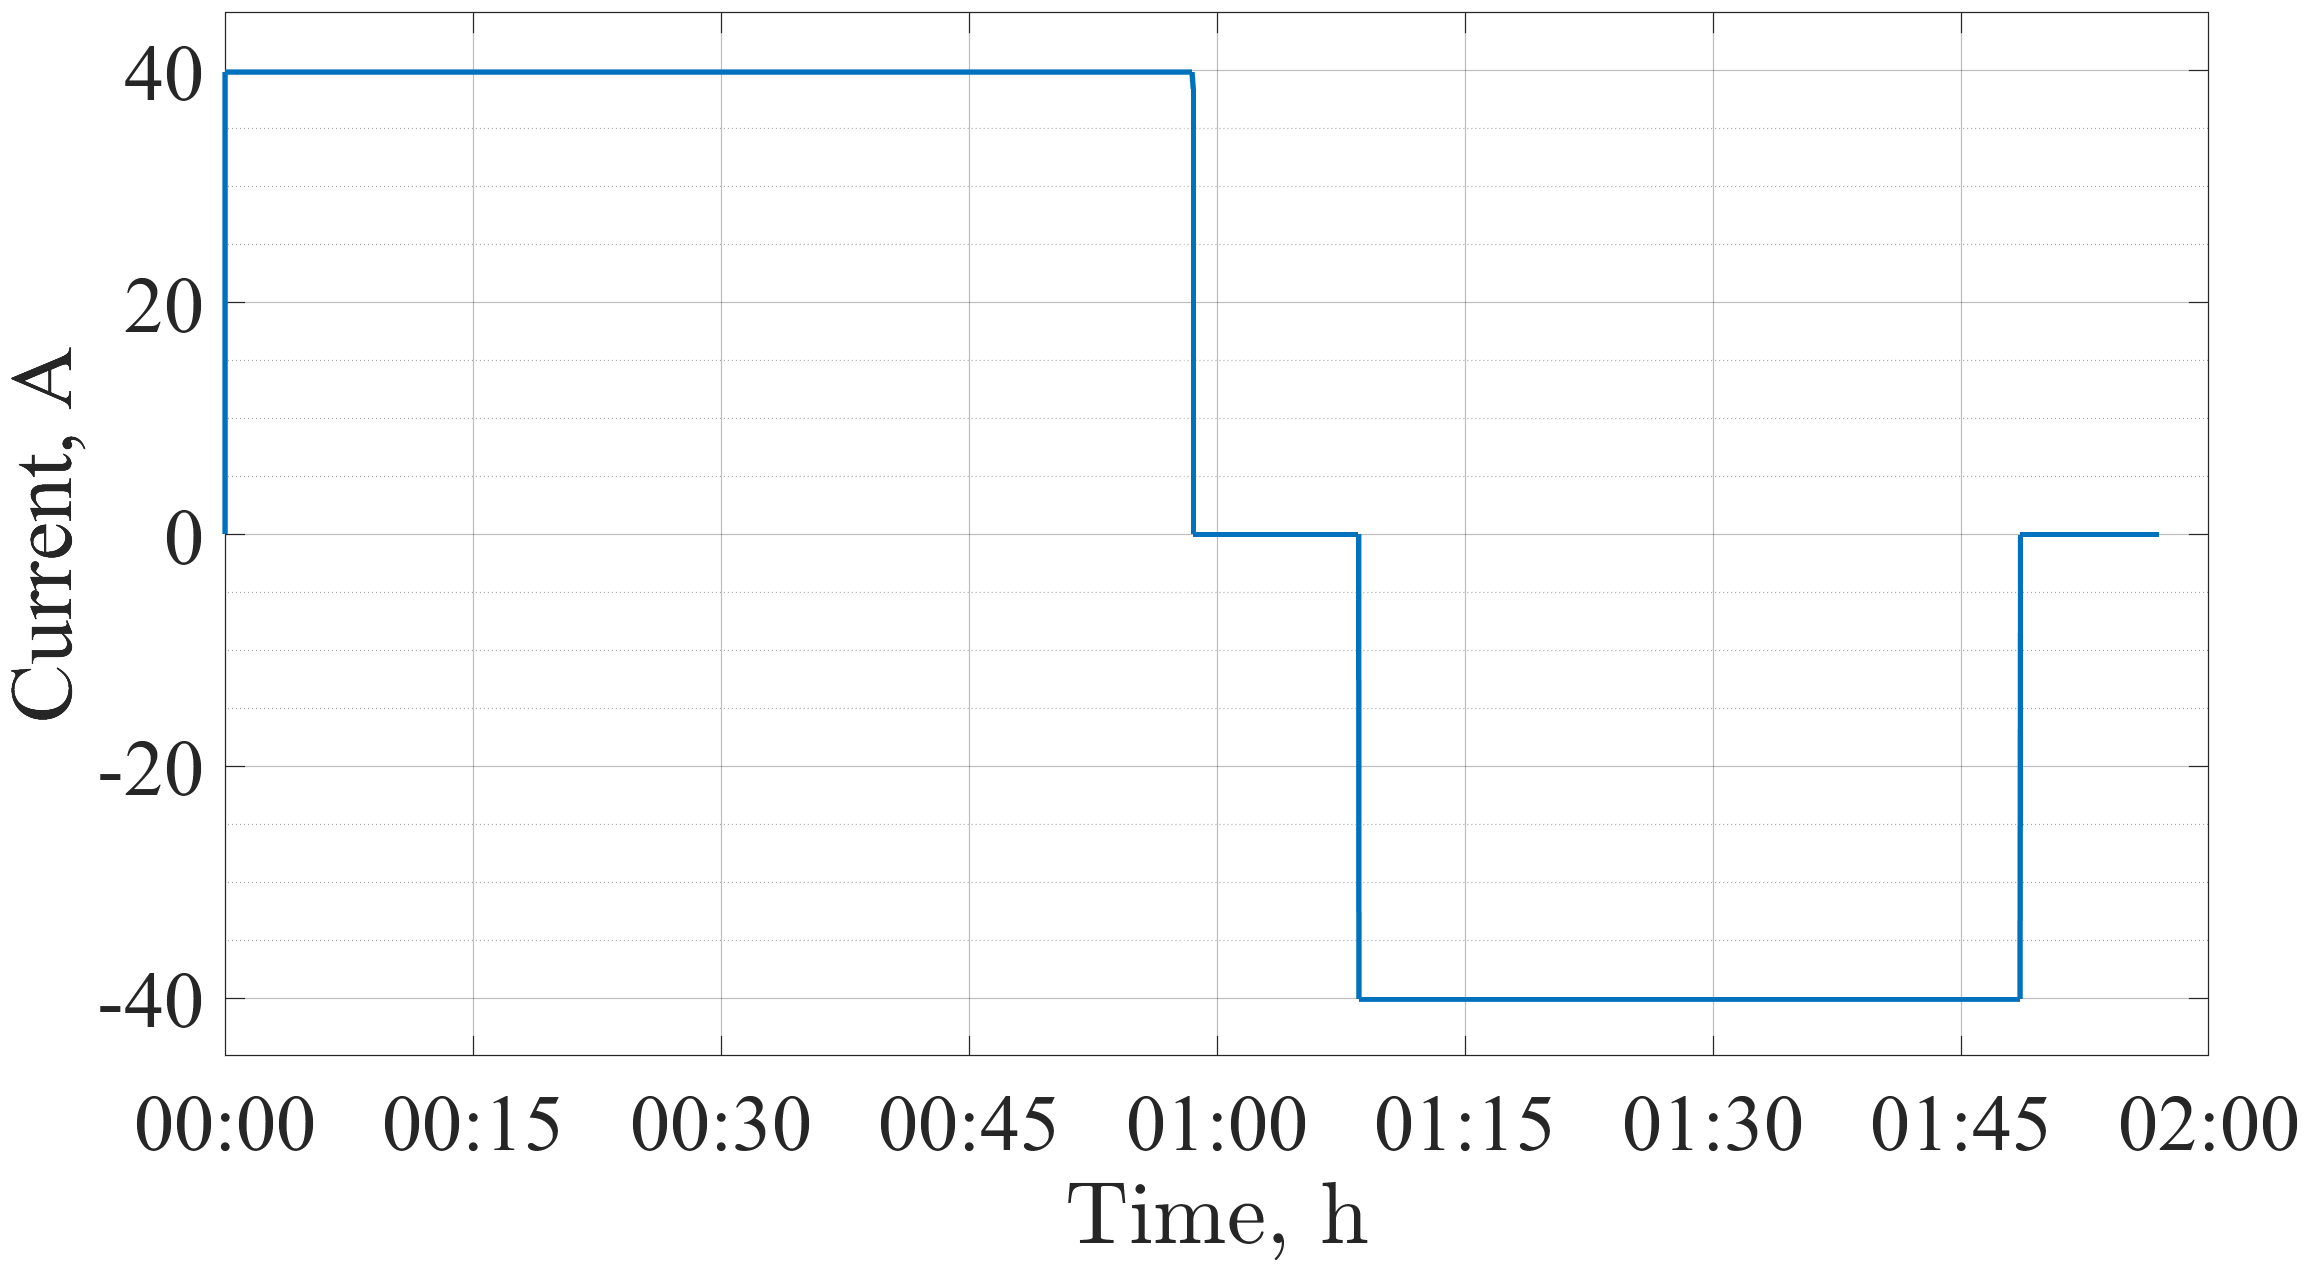
\includegraphics[scale=0.25]{statprofile_i}
    }
    \caption{Static current profile.}\label{fig:statprofile_i}
\end{figure}
\begin{figure}[ht]
    \centerfloat{
        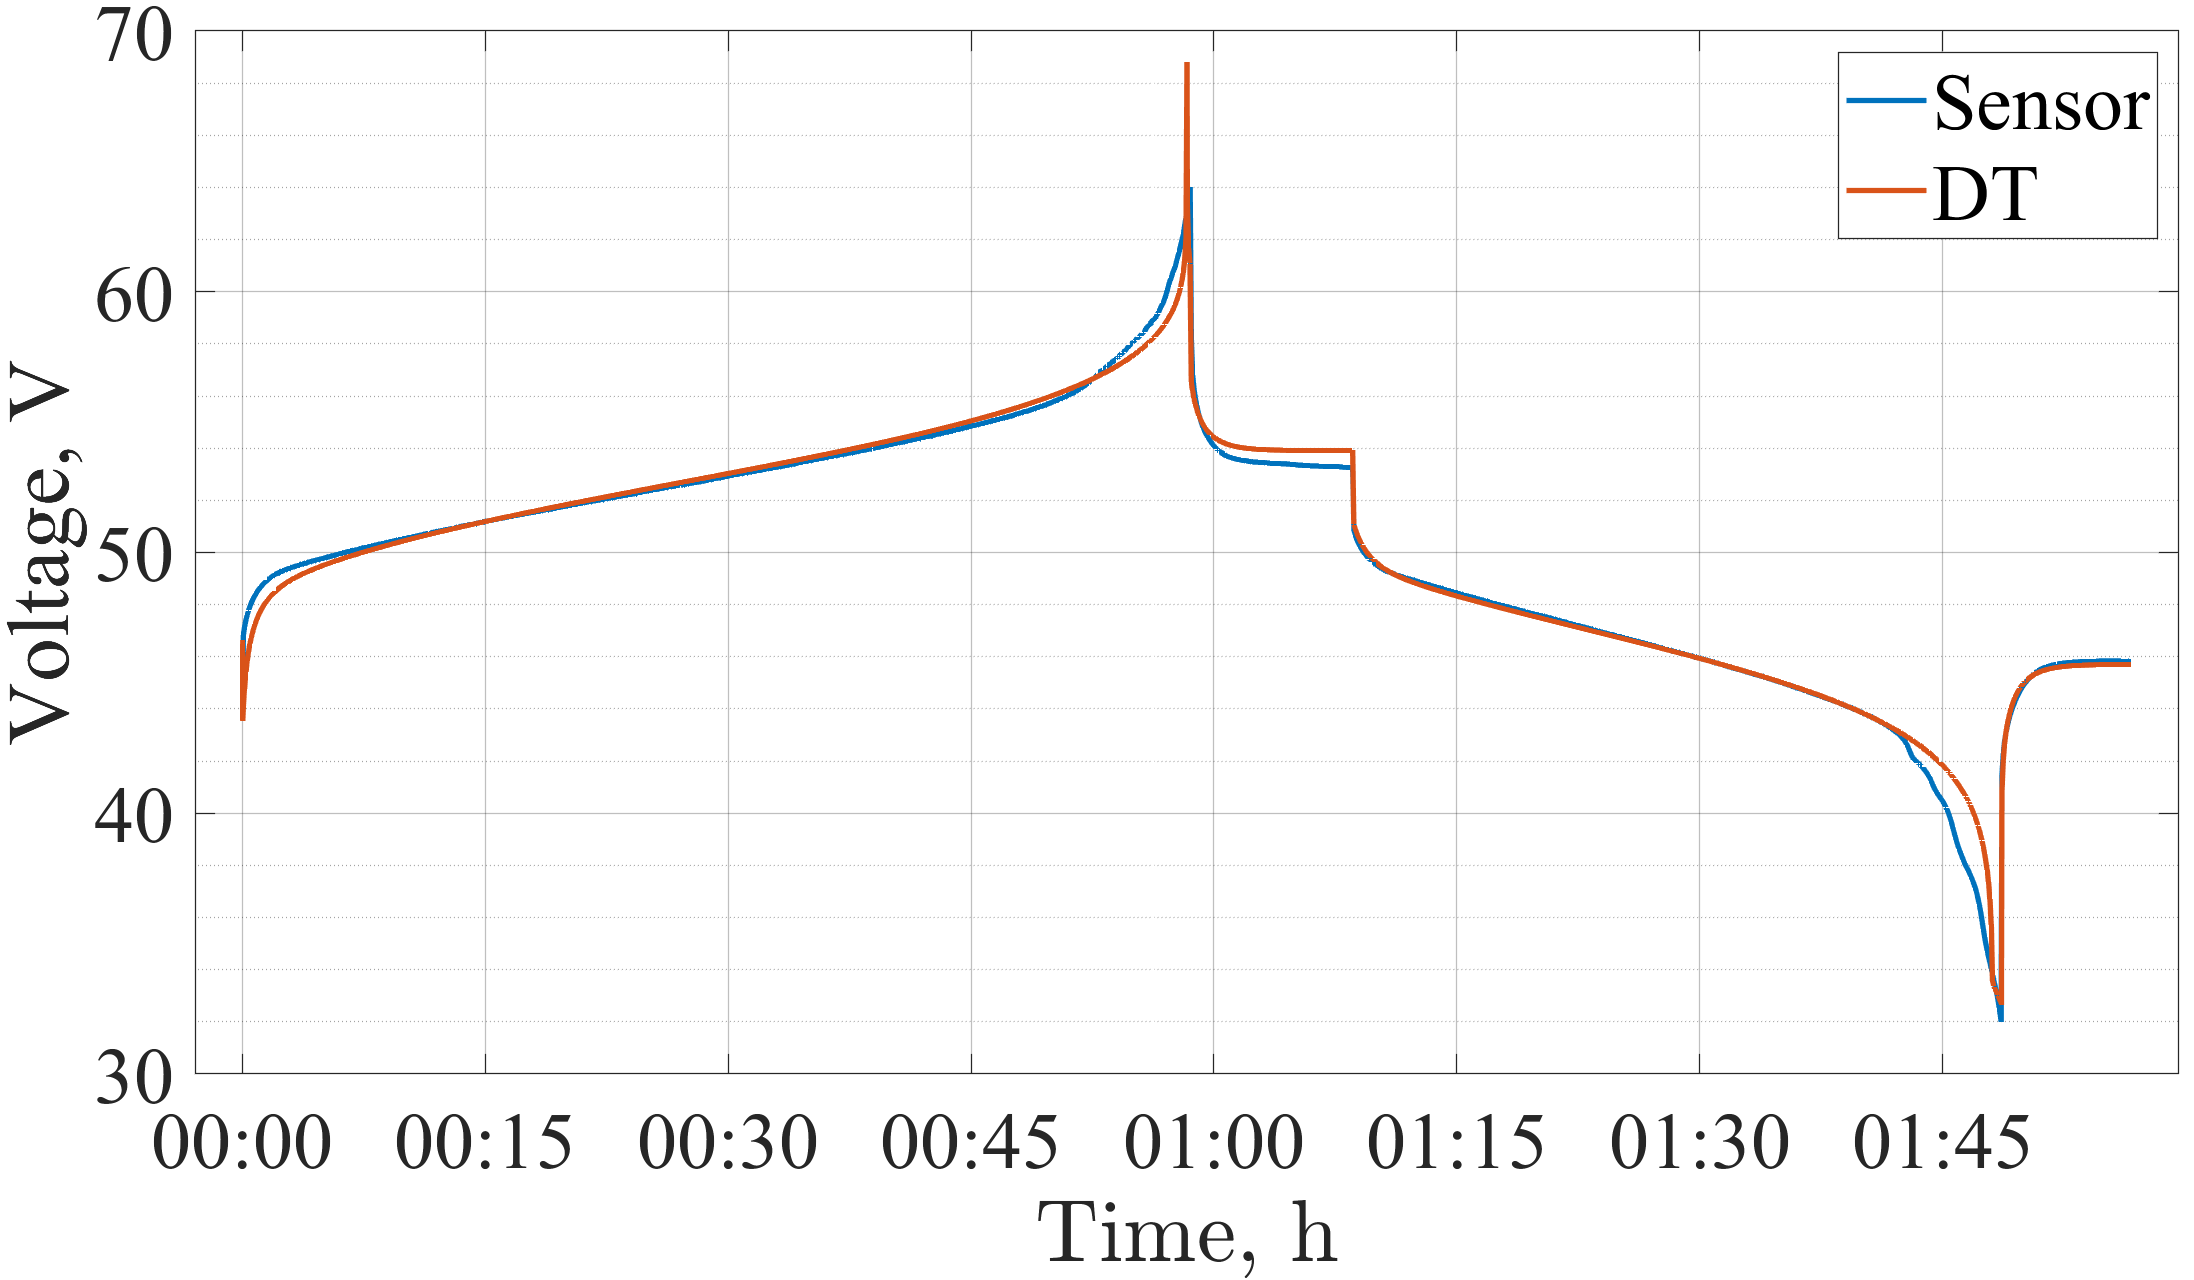
\includegraphics[scale=0.25]{statprofile_v}
    }
    \caption{Voltage response to static current profile.}\label{fig:statprofile_v}
\end{figure}
\begin{figure}[ht]
    \centerfloat{
        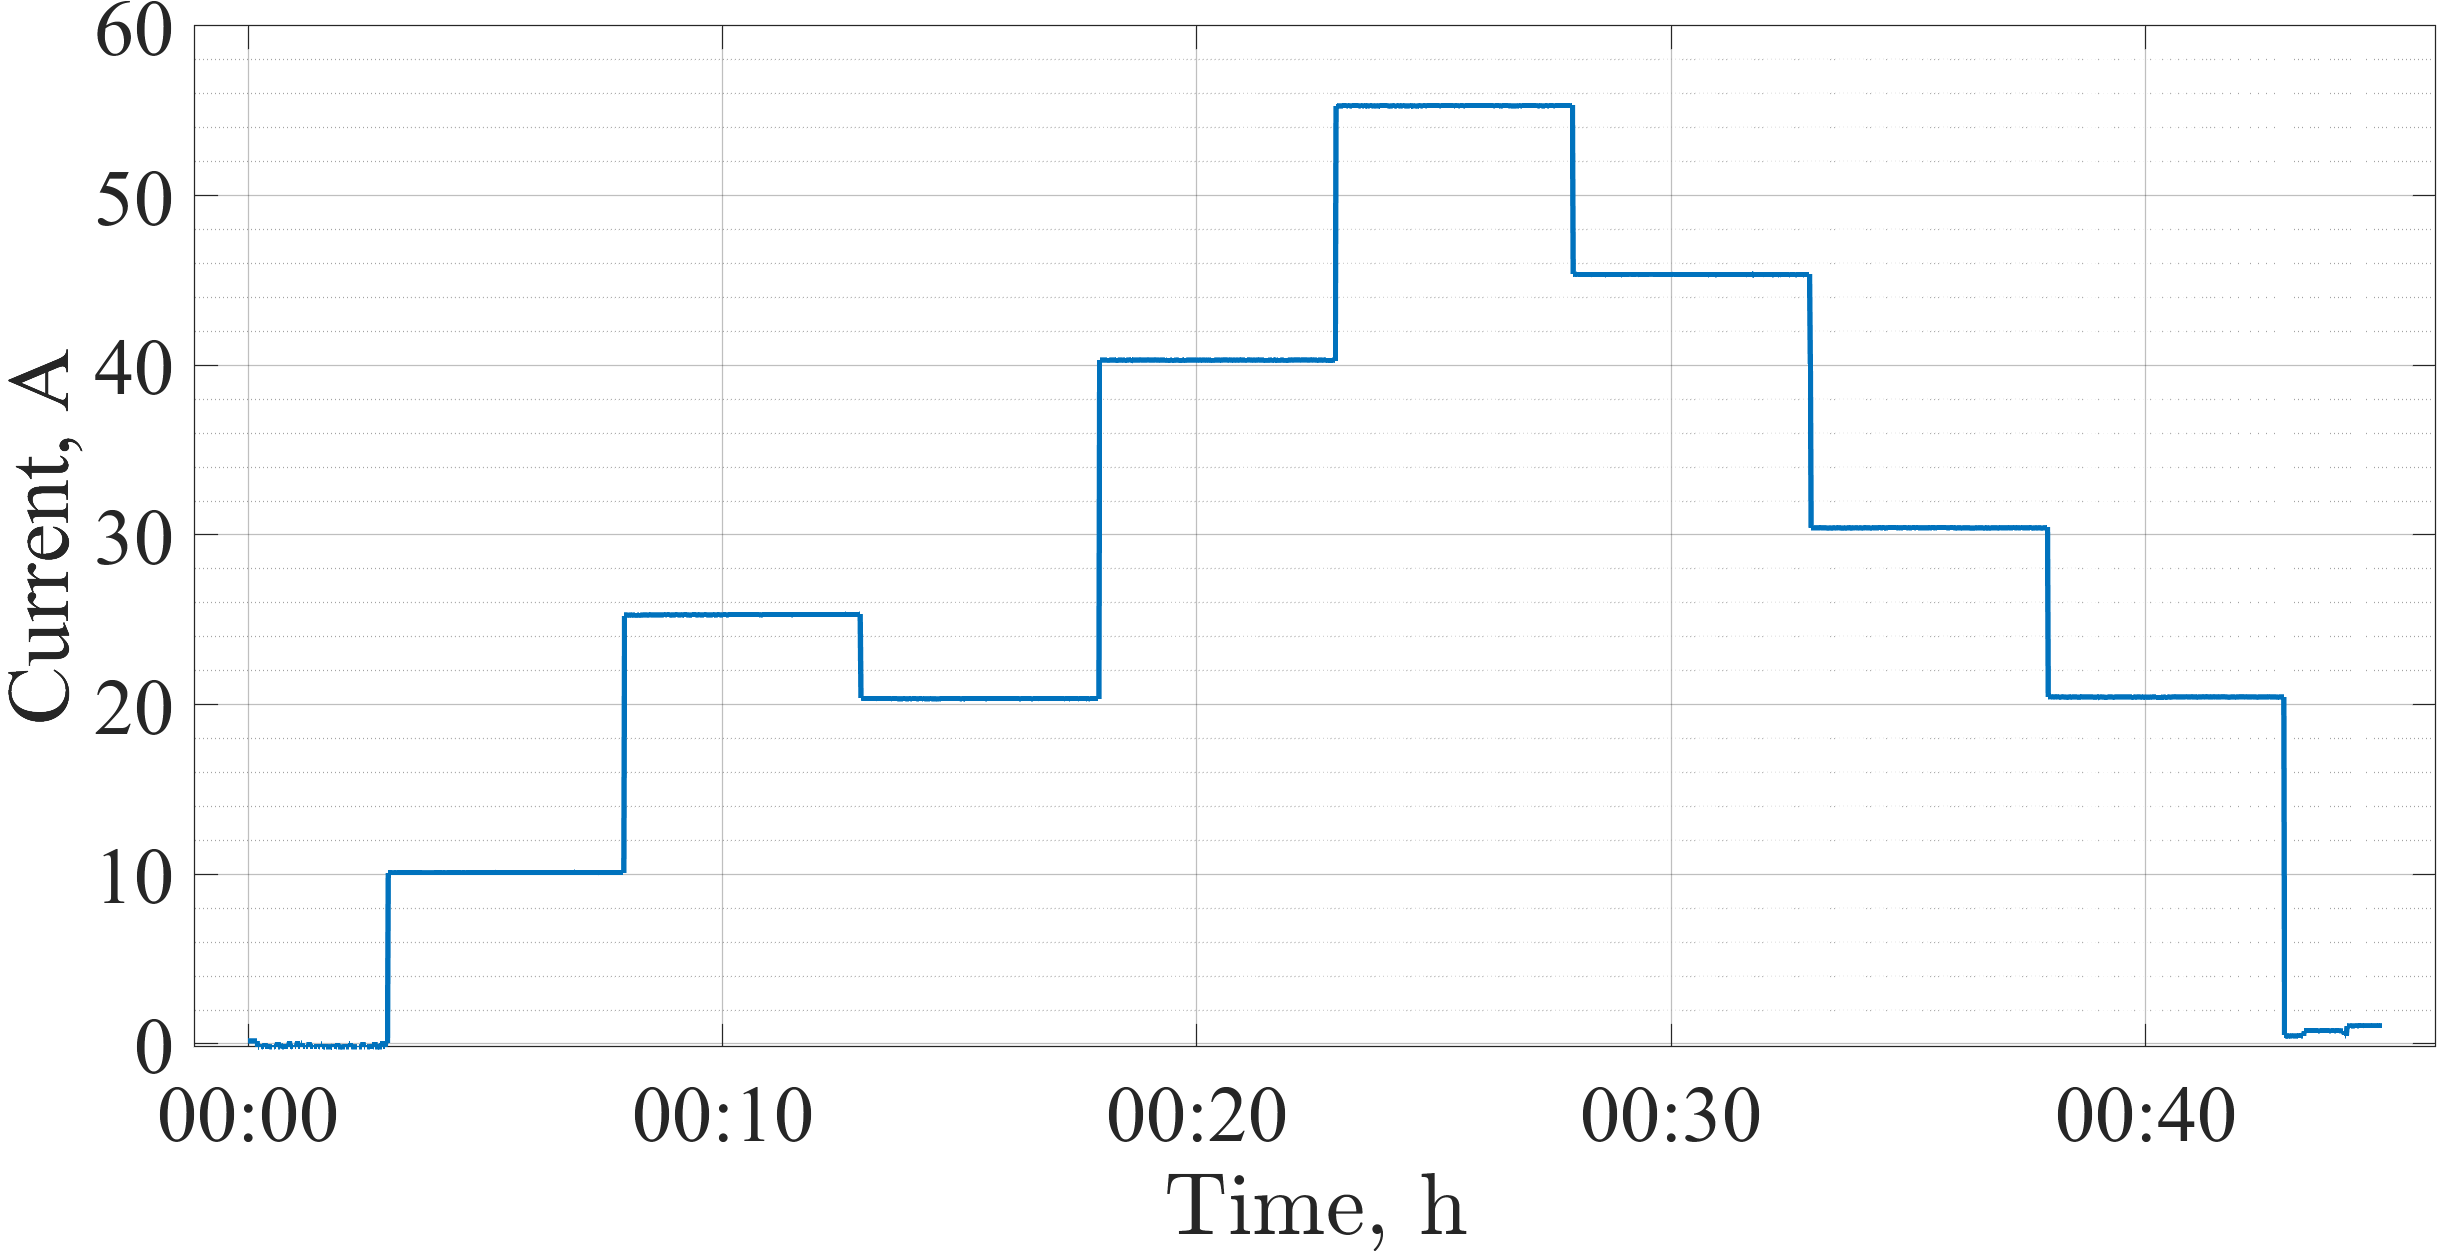
\includegraphics[scale=0.23]{dynprofile_i}
    }
    \caption{Multi-step constant current current profile.}\label{fig:dynprofile_i}
\end{figure}
\begin{figure}[ht]
    \centerfloat{
        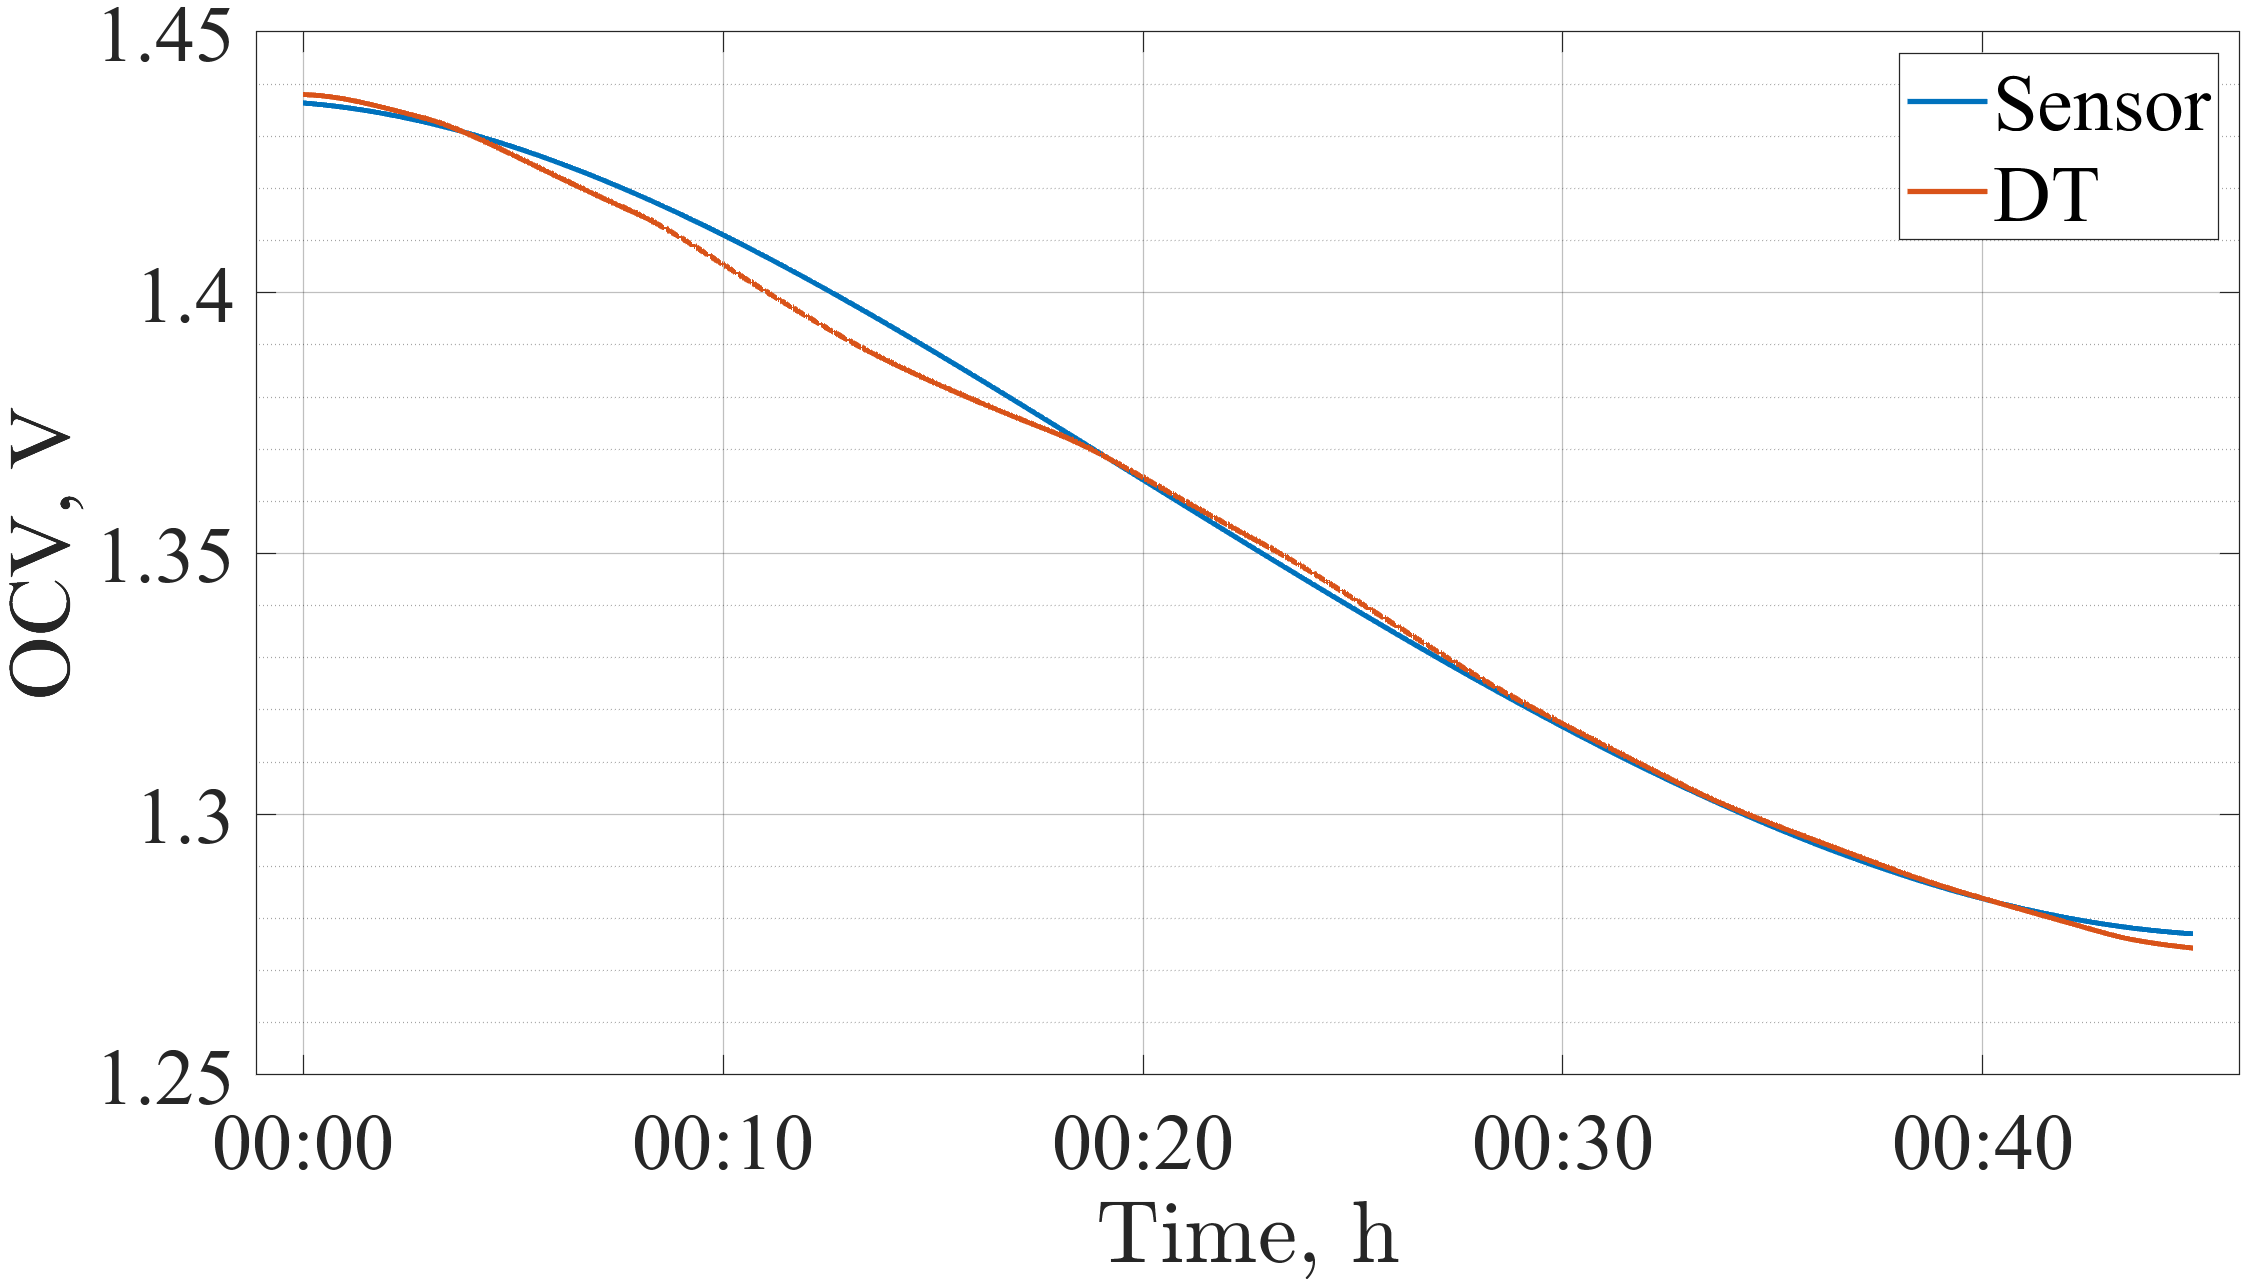
\includegraphics[scale=0.25]{dynprofile_ocv}
    }
    \caption{Inlet OCV response to multi-step constant current profile.}\label{fig:dynprofile_ocv}
\end{figure}
\begin{figure}[ht]
    \centerfloat{
        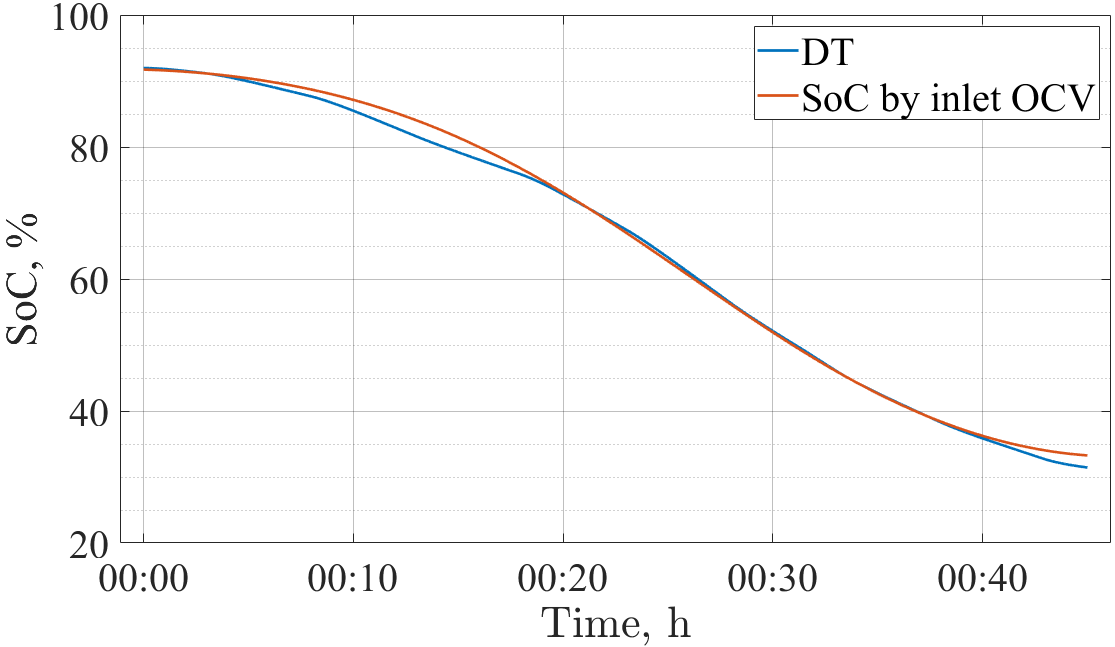
\includegraphics[scale=0.5]{dynprofile_soc2}
    }
    \caption{SoC change during multi-step constant current profile.}\label{fig:dynprofile_soc2}
\end{figure}
\begin{figure}[ht]
    \centerfloat{
        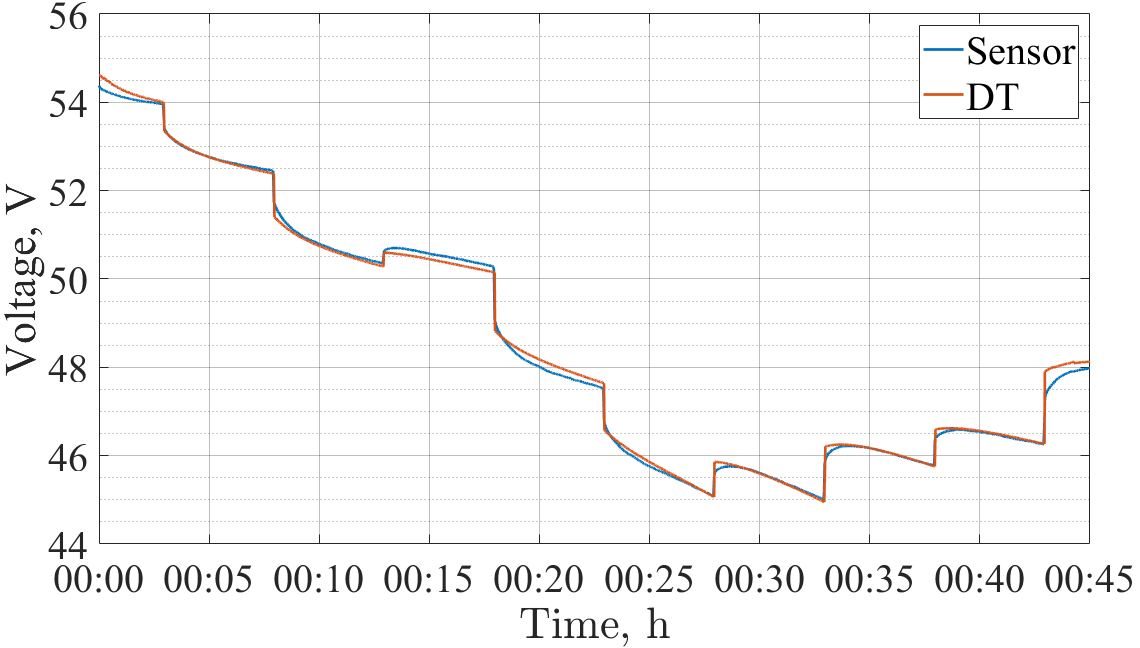
\includegraphics[scale=0.5]{dynprofile_v}
    }
    \caption{Voltage change during multi-step constant current profile.}\label{fig:dynprofile_v}
\end{figure}

\textbf{DT for PEDG validation}. To validate the described approach, the physical grid and digital twin were realized on the basis of the proved HIL approach according to the physical asset structure, shown in Figure~\cref{fig:rt_test_bench}. DT is implemented as real-time model within a separate computational device. For the lab application, we have used a real-time simulator (OPAL-RT 5600), but it can be implemented on any digital signal processor or edge devices. To accurately reflect the voltage dynamics of the physical grid, the DT leverages analog-to-digital boards within the OPAL-RT system to receive analog signals from the "real" microgrid, which is emulated by the RTDS simulator.

\begin{figure}[htbp]
    \centering
    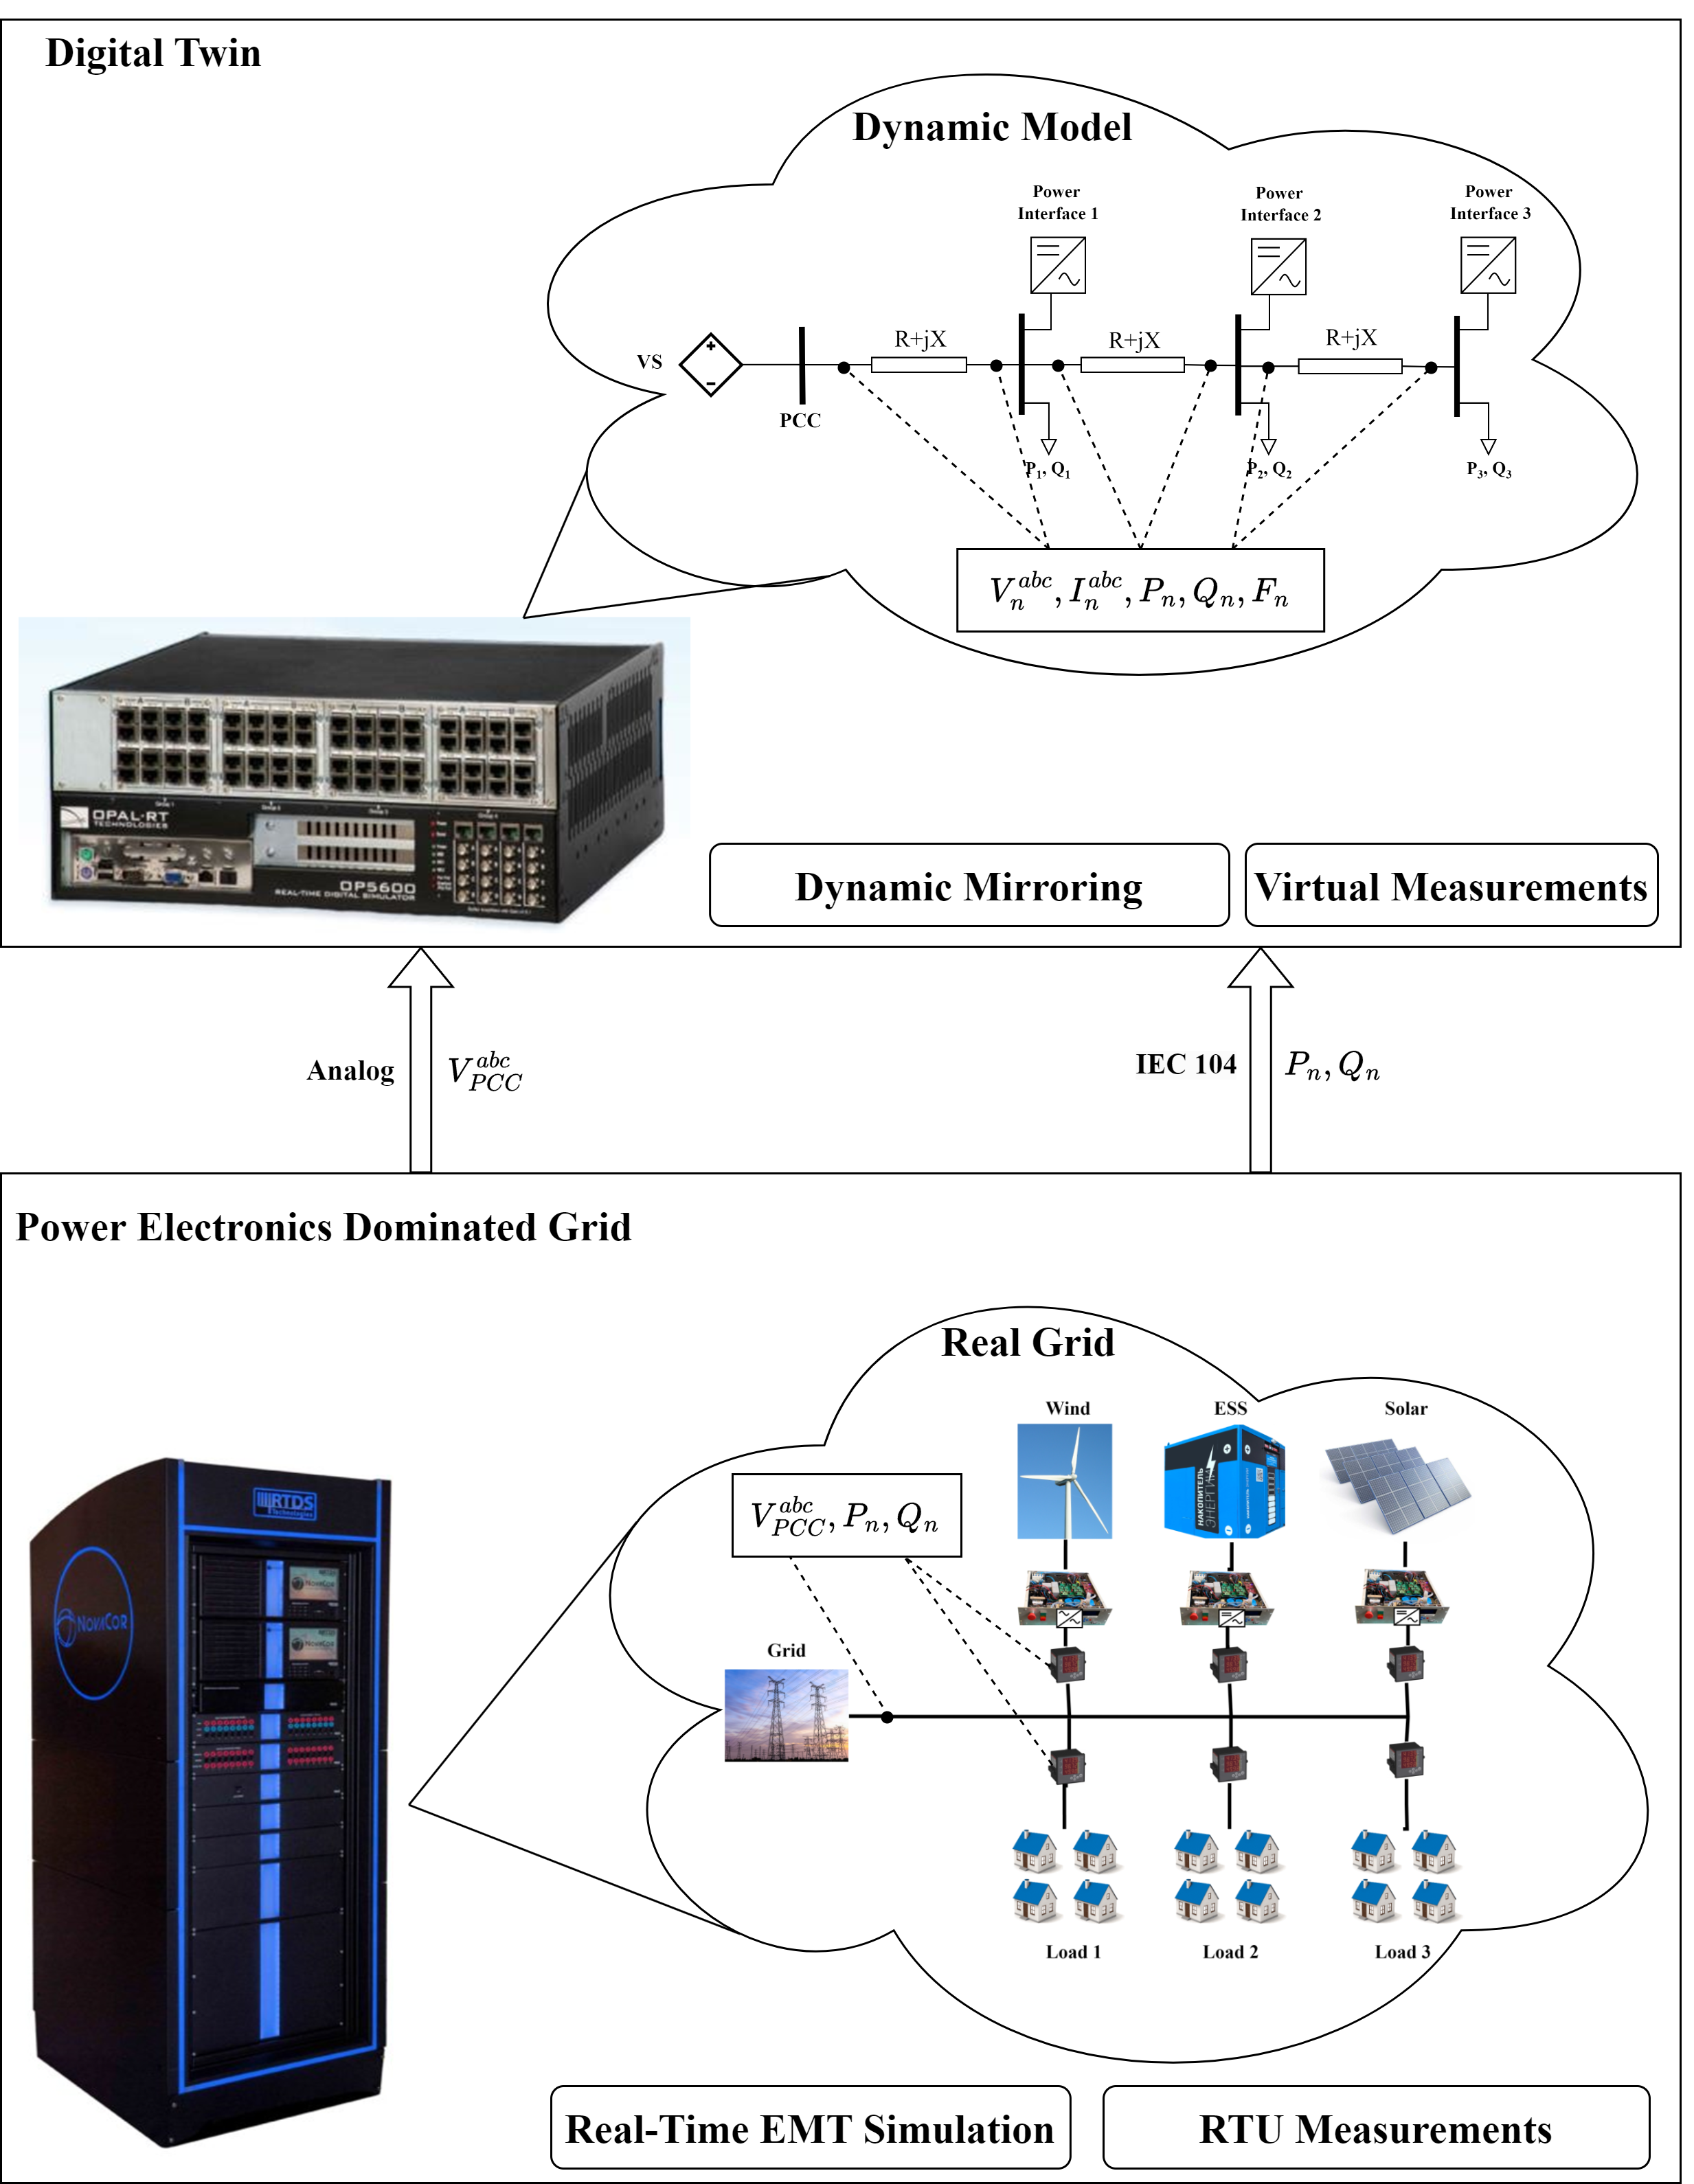
\includegraphics[width = 1\columnwidth]{test_bench.png}
    \caption{Hardware-in-the-loop test bench system for DT based dynamic mirroring.}
    \label{fig:rt_test_bench}
\end{figure}

For enhanced monitoring, protection and control, synchronized wave-formed data is preferred \autocite{Xu_Huang_Xie_Li_2022}. However, this can result in an overload of the data transmission system. Consequently, an integrated measurement system has been implemented in which the three-phase sinusoidal signal $V_{abc}$ is measured at the PCC, and $P$ and $Q$ are obtained at each POC of electricity sources, loads or prosumers. The values $P$ and $Q$ are received from the remote terminal units (RTU) by the IEC 60870-5-104 protocol and collected by OPC server. Integrating these measurement datasets within the precise DT model enables the observation of synchronized wave-formed data for voltages and currents across the entire feeder at any given point. In the same time, the usage fast analog measurements from only one point allow to avoid computational and informational complexity within scaling of the grid.

To validate the precision of the DT estimating dynamic states, the response to variations in voltage and frequency due to changes in power flow or frequency deviation of the grid were examined. At the head of the feeder, the system starts in a balanced condition where both the frequency and voltage are considered at their nominal values. 

At 10 seconds, the voltage at the POC of the loads $1$ and $3$ deviates from its nominal level due to changes in power injection and consumption according power curve in Figure~\cref{fig:p_response}. Figure~\cref{fig:v_response} illustrates the voltage transients occurring during power flow load changes at PCC. Figure~\cref{fig:f_response} illustrates the frequency deviations measured in load $1$ caused by a change in the frequency of the external grid generator. The droop coefficient for the external grid generator set is relatively small to be sensitive to load variation within the microgrid. The voltage and frequency response in the digital twin estimator shows good accuracy with small difference that is considered negligible and has no significant impact on overall performance or system operation.

\begin{figure}[htbp]
    \centering
    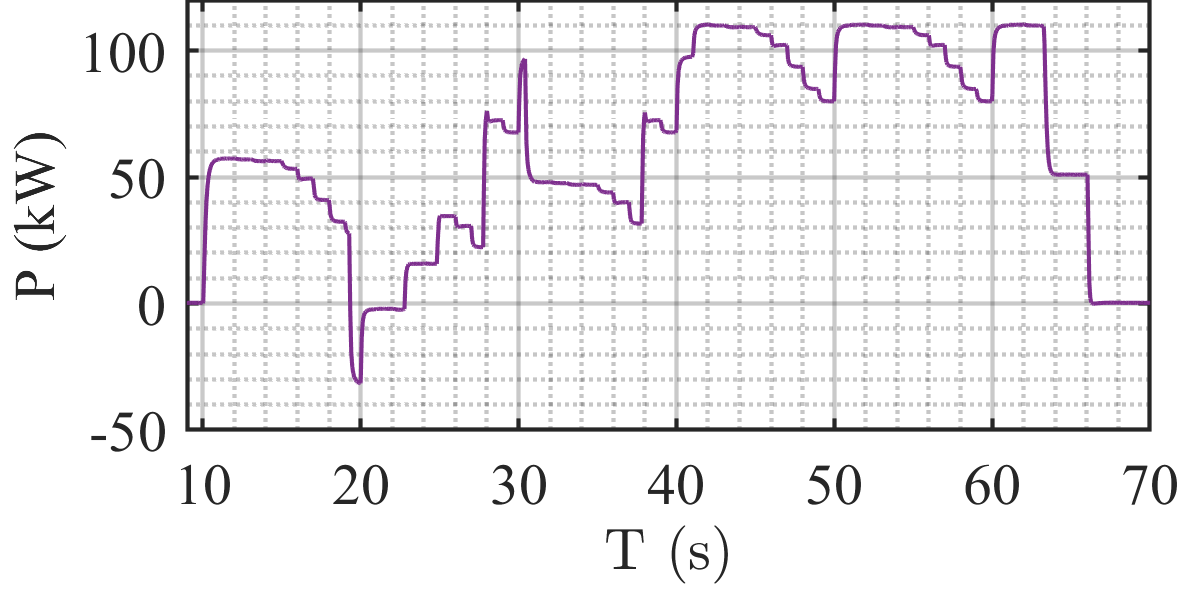
\includegraphics[width = 0.8\columnwidth]{p_5.png}
    \caption{Power transient at the point at the point of common coupling.}
    \label{fig:p_response}
\end{figure}
\begin{figure}[htbp]
    \centering
    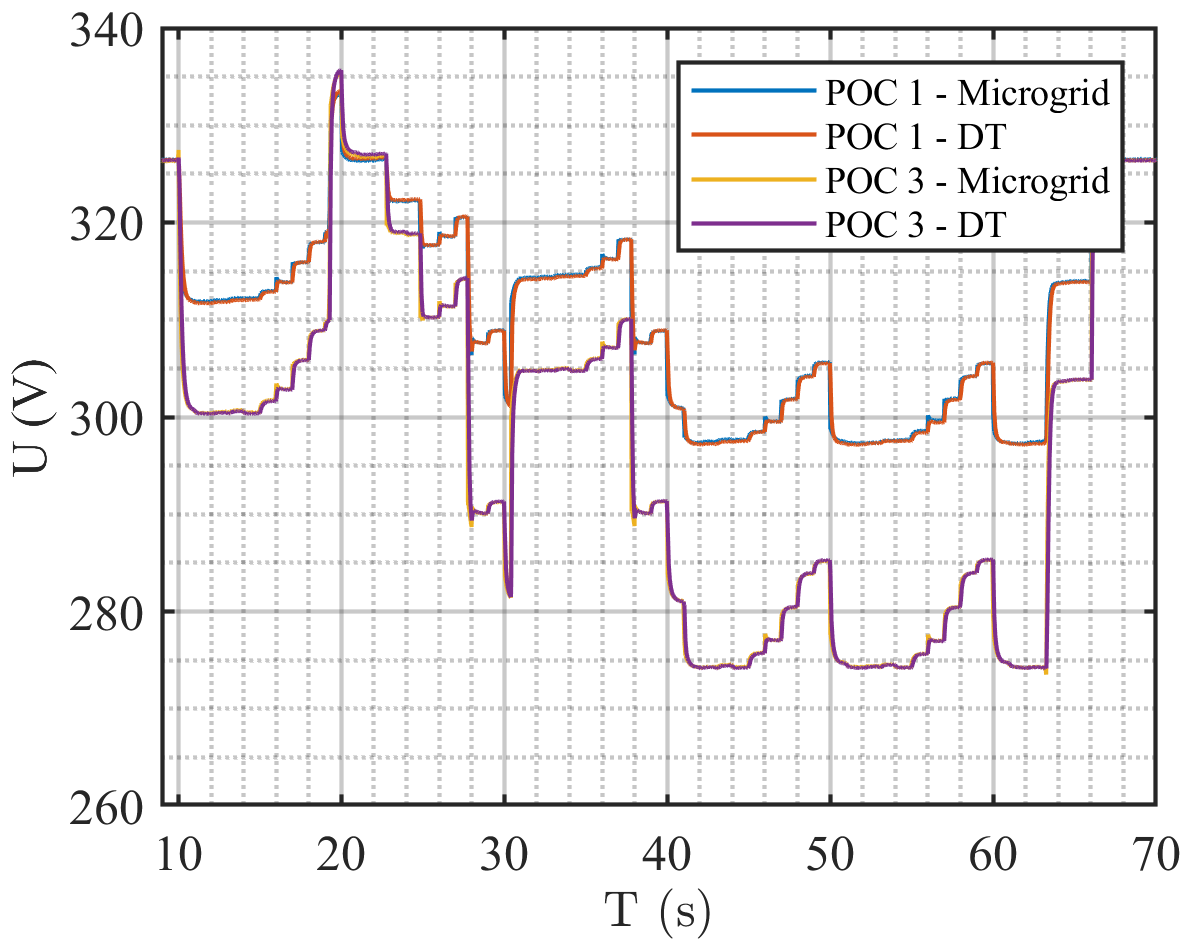
\includegraphics[width = 0.8\columnwidth]{v_7.png}
    \caption{Voltage transient response of loads 1 and 3 at point of connection.}
    \label{fig:v_response}
\end{figure}
\begin{figure}[htbp]
    \centering
    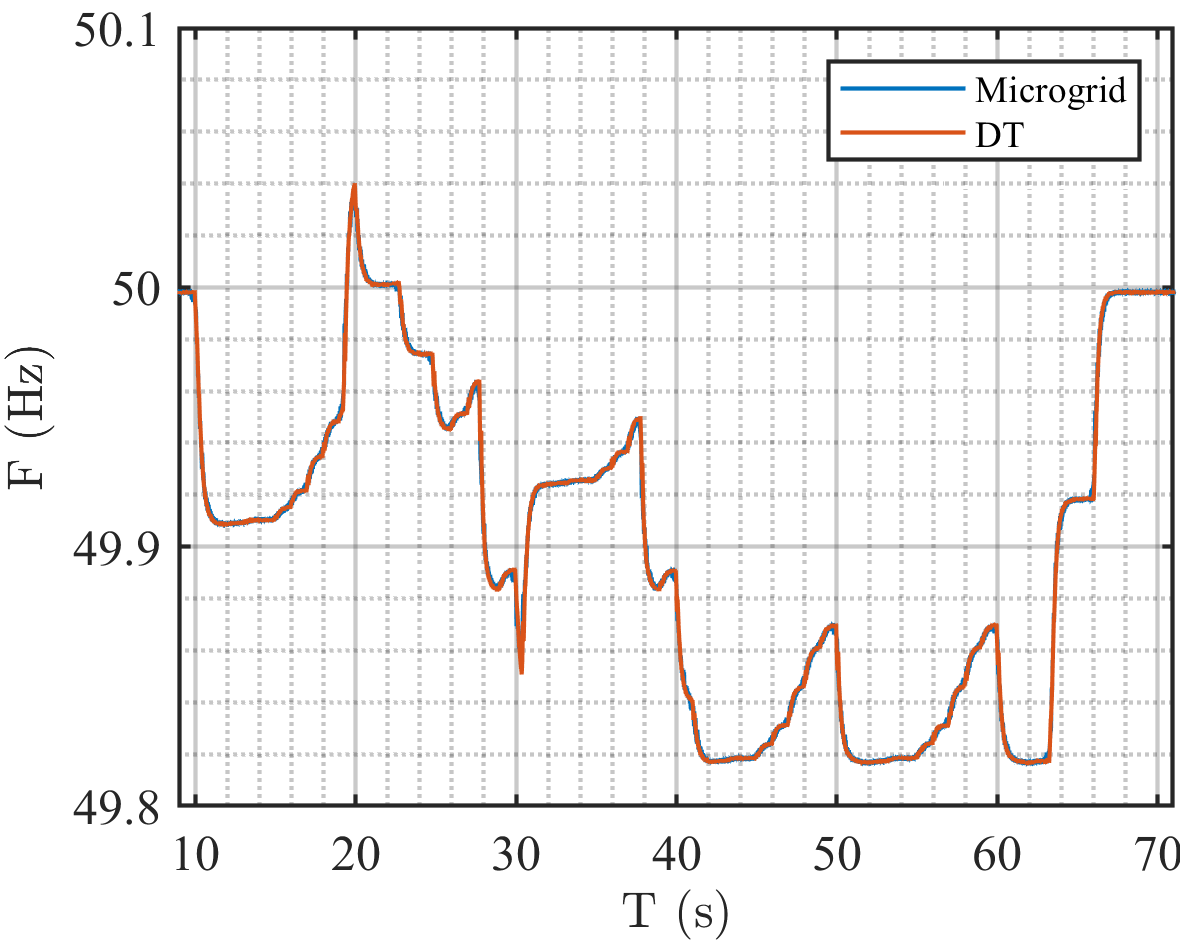
\includegraphics[width = 0.8\columnwidth]{f_6.png}
    \caption{Frequency transient response of load 1 at point of connection.}
    \label{fig:f_response}
\end{figure}

\section{Impact of parameter deviations}\label{sec:ch4/sec4}
One critical aspect that often requires thorough investigation is the sensitivity of digital twins to variations in the model parameters. In practical scenarios, the parameters of microgrid participants can deviate from their expected values due to a number of factors, including environmental conditions, operational changes, and unforeseen contingencies. Such discrepancies can lead to significant deviations between the digital twin's predictions and the actual performance of the microgrid. However, through continuous monitoring and analysis of real-time data, the digital twin can detect when there is a considerable difference between the model and reality. Leveraging its set of measurements and advanced analytics, the DT can autonomously perform corrective actions, such as triggering alarms, adjusting parameters to better align with observed conditions, and notifying users of potential issues. 

The greatest impact can be made by power inverters as it has complex dynamics and obviously time delays that can arise due to various reasons, such as control system latency, communication lags, or even physical distance between components. In addition, factors such as aging and manufacturing variability can lead to degradation and a variety of components, such as filter inductance quality. Environmental conditions may necessitate tuning the operational mode and adjusting PI controllers in PLL and the current control loop in the physical device, causing deviations from the DT model.

In this study, we assessed the sensitivity of the DT due to variations in parameters affecting the inverter dynamics between the physical asset and the DT model, specifically the PI controller in the PLL, the PI controller of the current control loop, and the filter inductance. The inverter output voltage at the POC was compared between the DT and the real grid model using a fixed data transfer rate of 10 $ms$. The error was defined as:

\begin{equation}
     \xi(V_{poc}^{inv}) = Y_{DT}(P) - Y_{MG},
\end{equation}
where $P = P_n + \delta P$ represents the actual parameter values with deviations. $P_n$ is the subset of parameters affecting inverter dynamics and communication time delay, including $K_p^{pll}, K_i^{pll}$ - proportional and integral part of the PLL's PI controller, $K_p^{cc}, K_i^{cc}$ - proportional and integral part of the current control loop's PI controller, $L_f$ - filter inductance, $\delta\tau$ - communication delay. 

Our findings in Figure~\cref{fig:s_all} indicate that deviations with 40\% from the nominal in control parameters ($K_i^{cc}, K_p^{pll}, K_i^{pll}$) and output filter ($L_f$) do not significantly affect the error. Inaccuracy in estimating the voltage level in the PCC after a load step do not exceed 200 $mV$. Unlike the current control proportional gain ($K_p^{cc}$), the deviation of which, according Figure~\cref{fig:s_cc},  result in greater errors in the voltage level, potentially reaching nearly 1 $V$. These findings underscore the critical importance of precise tuning in the current control loop to maintain the accuracy of the state estimation.

\begin{figure}[htbp]
    \centering
    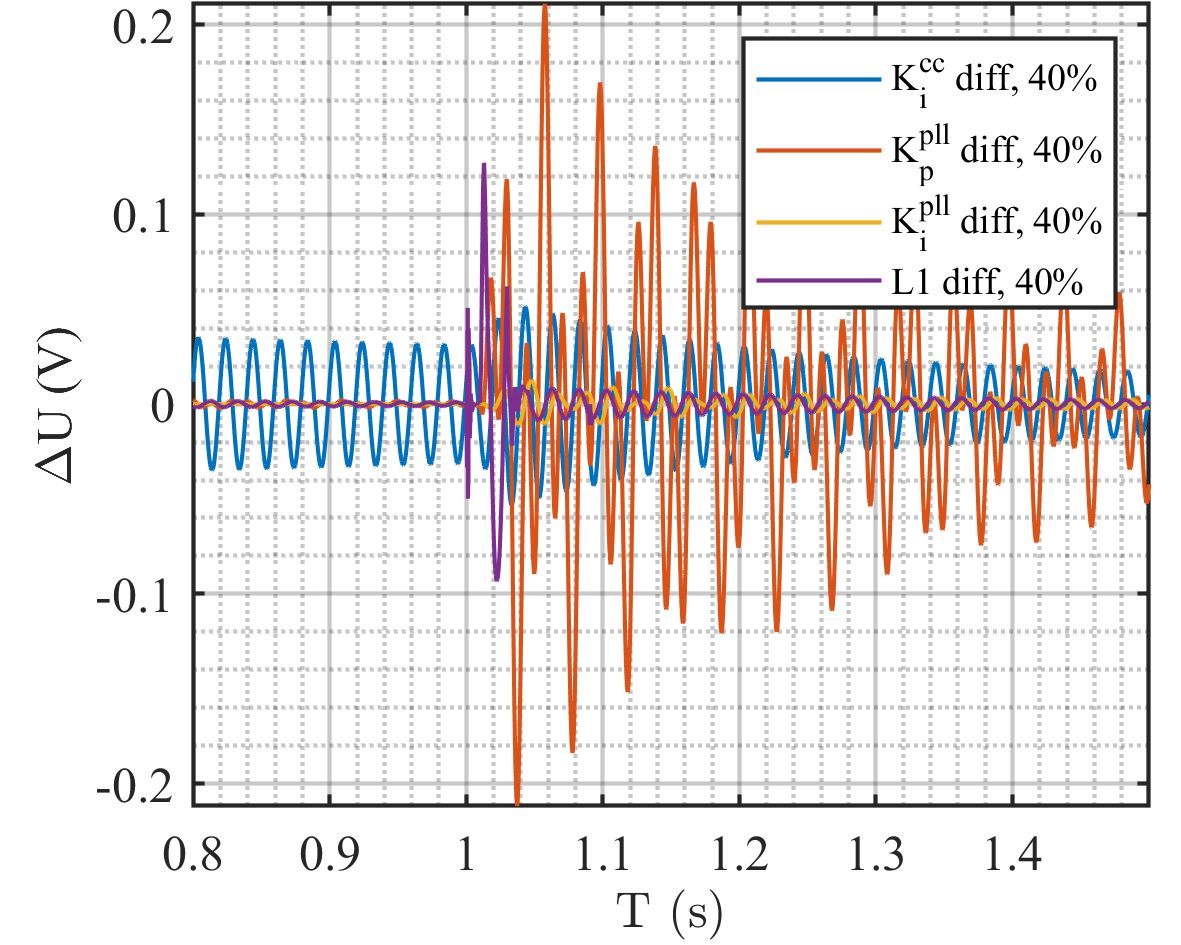
\includegraphics[width = 0.8\columnwidth]{all2.png}
    \caption{Voltage error deviation affected by main controller dynamics parameters inequality.}
    \label{fig:s_all}
\end{figure}
\begin{figure}[htbp]
    \centering
    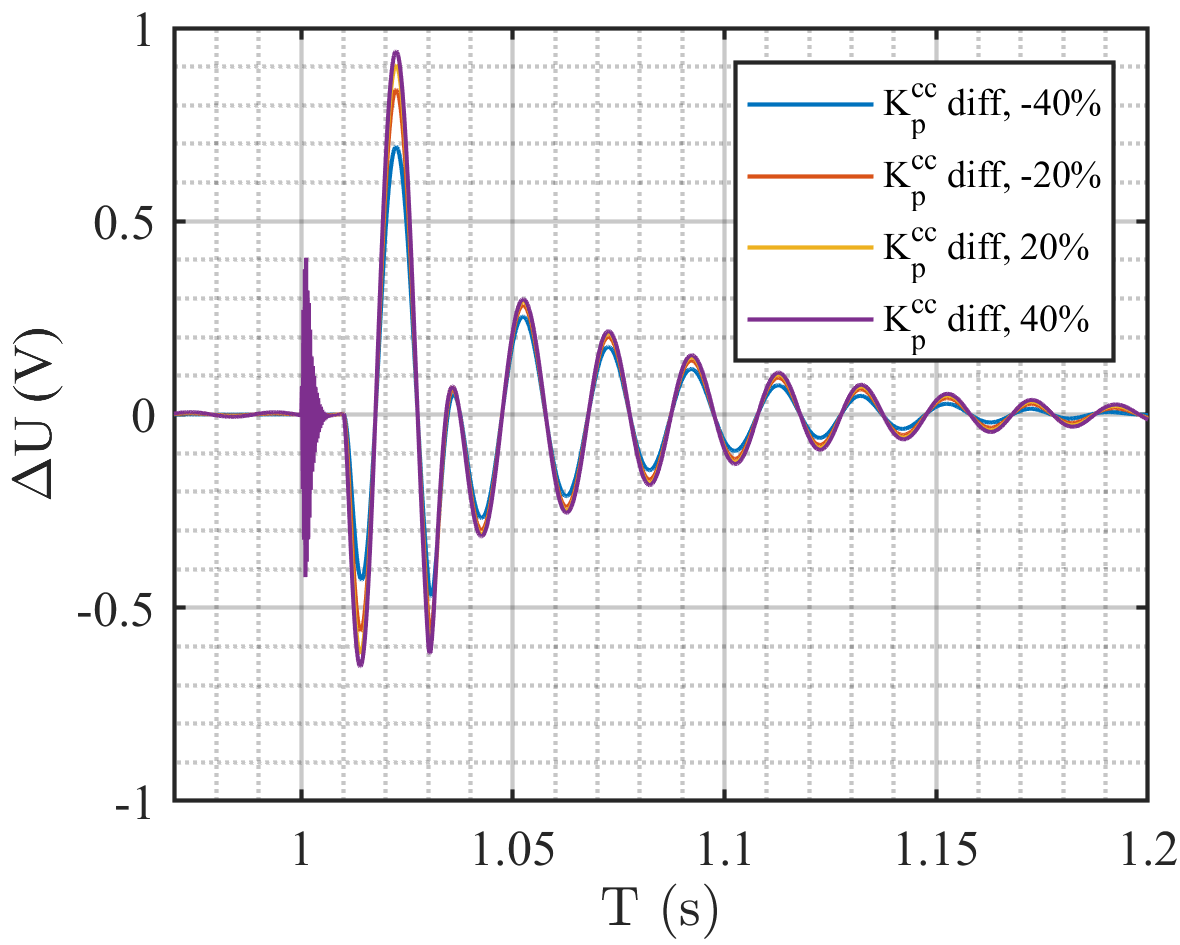
\includegraphics[width = 0.8\columnwidth]{cc_kp4.png}
    \caption{Voltage error deviation affected by proportional part of current control loop parameter inequality.}
    % $K_p^{cc}$ 
    \label{fig:s_cc}
\end{figure}
\begin{figure}[htbp]
    \centering
    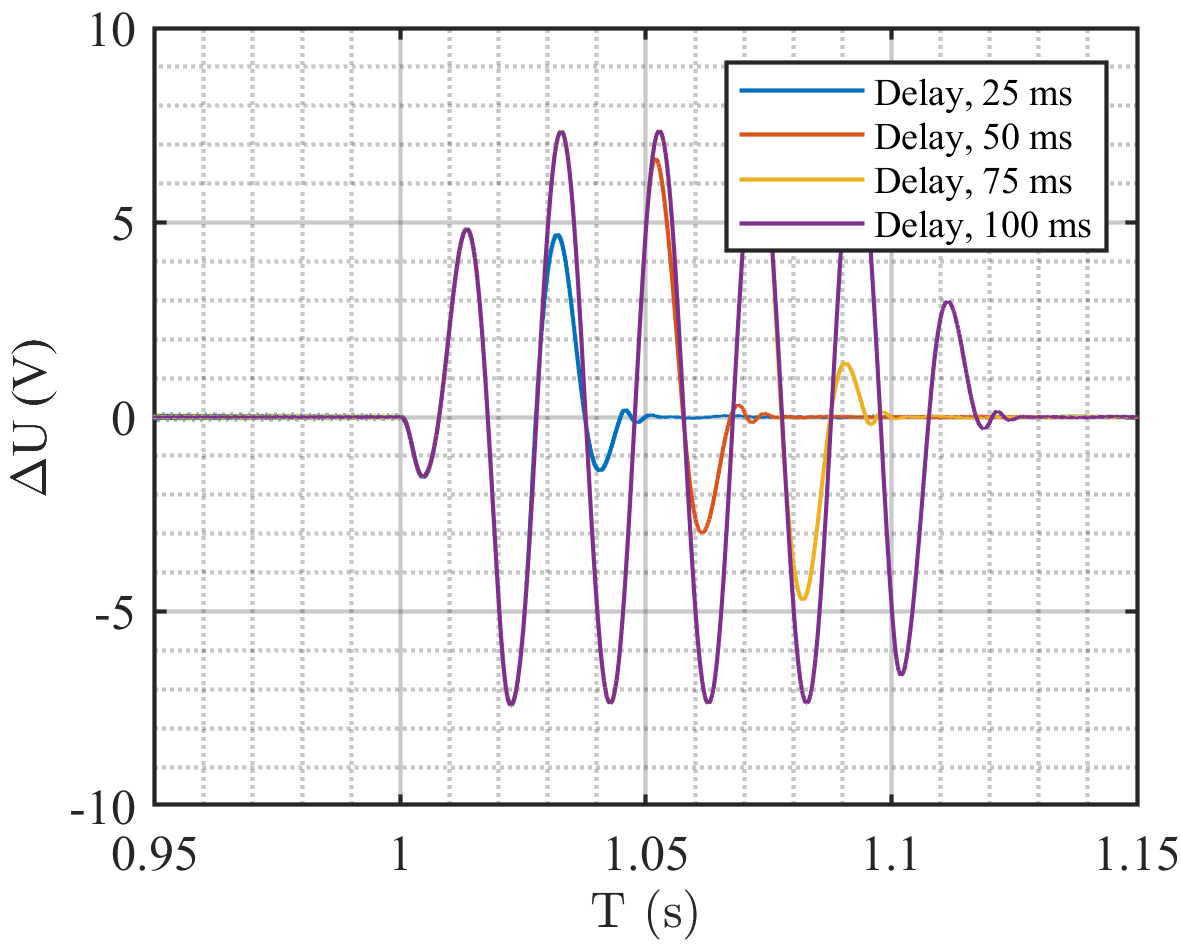
\includegraphics[width = 0.8\columnwidth]{meas_delay3.png}
    \caption{Voltage error deviation affected by measurement data transfer delay.}
    \label{fig:s_md}
\end{figure}
\begin{figure}[htbp]
    \centering
    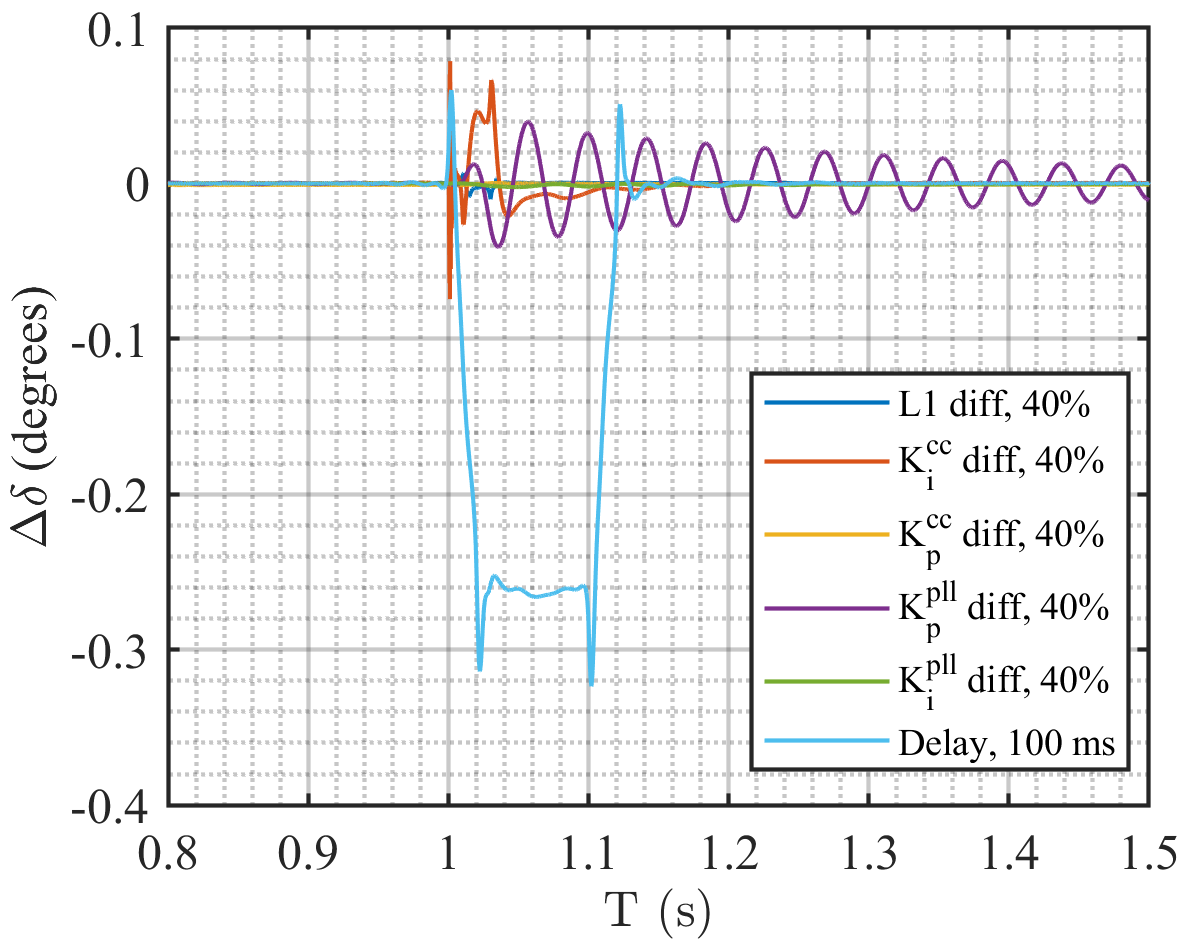
\includegraphics[width = 0.8\columnwidth]{phi2.png}
    \caption{Phase error deviation affected by main controller dynamics parameters inequality.}
    \label{fig:phi}
\end{figure}

Furthermore, the study reveals that hardware configurations and data handling practices significantly influence voltage stability. As shown in Figure~\cref{fig:s_md}, measurement delays, ranging from 50 to 200 $ms$, induce substantial voltage deviation errors of up to ±7 $V$ and setting time up to 0.1 $s$, highlighting the system's extreme sensitivity to data transfer rates. These results emphasize the necessity of minimizing measurement delays up to 10 ms.

The phase match also makes a significant contribution to the accuracy in DSE. From Figure~\cref{fig:phi} it is clear that the greatest impact comes from the data transfer delay and the PLL control loop, causing a deviation of about 0.3 degrees. With an apparent small deviation value, it can lead to an unacceptable operating point of a digital twin. The transmission system yields the power flow equations in its linear approximation (which is rather accurate for distribution grids) \autocite{machowski2020power}: 
\begin{equation}
    P_G = \frac{V_1 V_2}{X_L} \xi(\delta)
    \label{placeholder}
\end{equation}
where $P_G$ represents the power from the IBR. $V_1, V_2$ suggested as voltages directly after the IBR connection and after the transmission line. $X_L$ is reactive resistance of the transmission line. $\xi(\delta)$ represent an error between DT angle and real grid. Substituting 320 $V$ voltage level and 25 $m$ transmission line length within inductance equal to 0.0762 $H/km$ it can be obtained that within 0.3 degrees error the power mismatch will reach about 1 $kW$. This is 1$\%$ from the power level in the feeder head, but only if we take into account only one energy source. In case of hundreds of devices, this can lead to unacceptable inaccuracy of DT based state estimator.

\section{Anomaly Detection Validation}\label{sec:ch4/sec5}
To validate threat detection based on the collaborative work of DT and ML methods, the hardware-in-the-loop technique is utilized with a Man-in-the-middle (MITM) attack. The real microgrid structure is utilized as a detailed electromagnetic transient model within a real-time simulator (RTDS) representing consumers, solar generation, wind generation, and ESS with the appropriate power electronics interface. To reproduce real power flow, logged generation and consuming profiles are used in time as referenced values for power inverters and loads.  DT is represented by an average real-time model implemented in a separate real-time machine OPAL-RT 5600. To accurately reflect the state of the real grid, DT leverages sinusoidal analog voltages at the point of common coupling in the head of the feeder along with digital measurements transmitted from IED by IEC 60870-5-104 protocol. The measured power values received act as reference points for the loads and power inverters in the DT. This configuration guarantees that the overall DT model accurately represents the real-time condition of the physical asset simulated by the RTDS simulator. Figure~\cref{fig:mitm_bench} depicts this detailed test bench configuration.

\begin{figure}[ht]
    \centerfloat{
        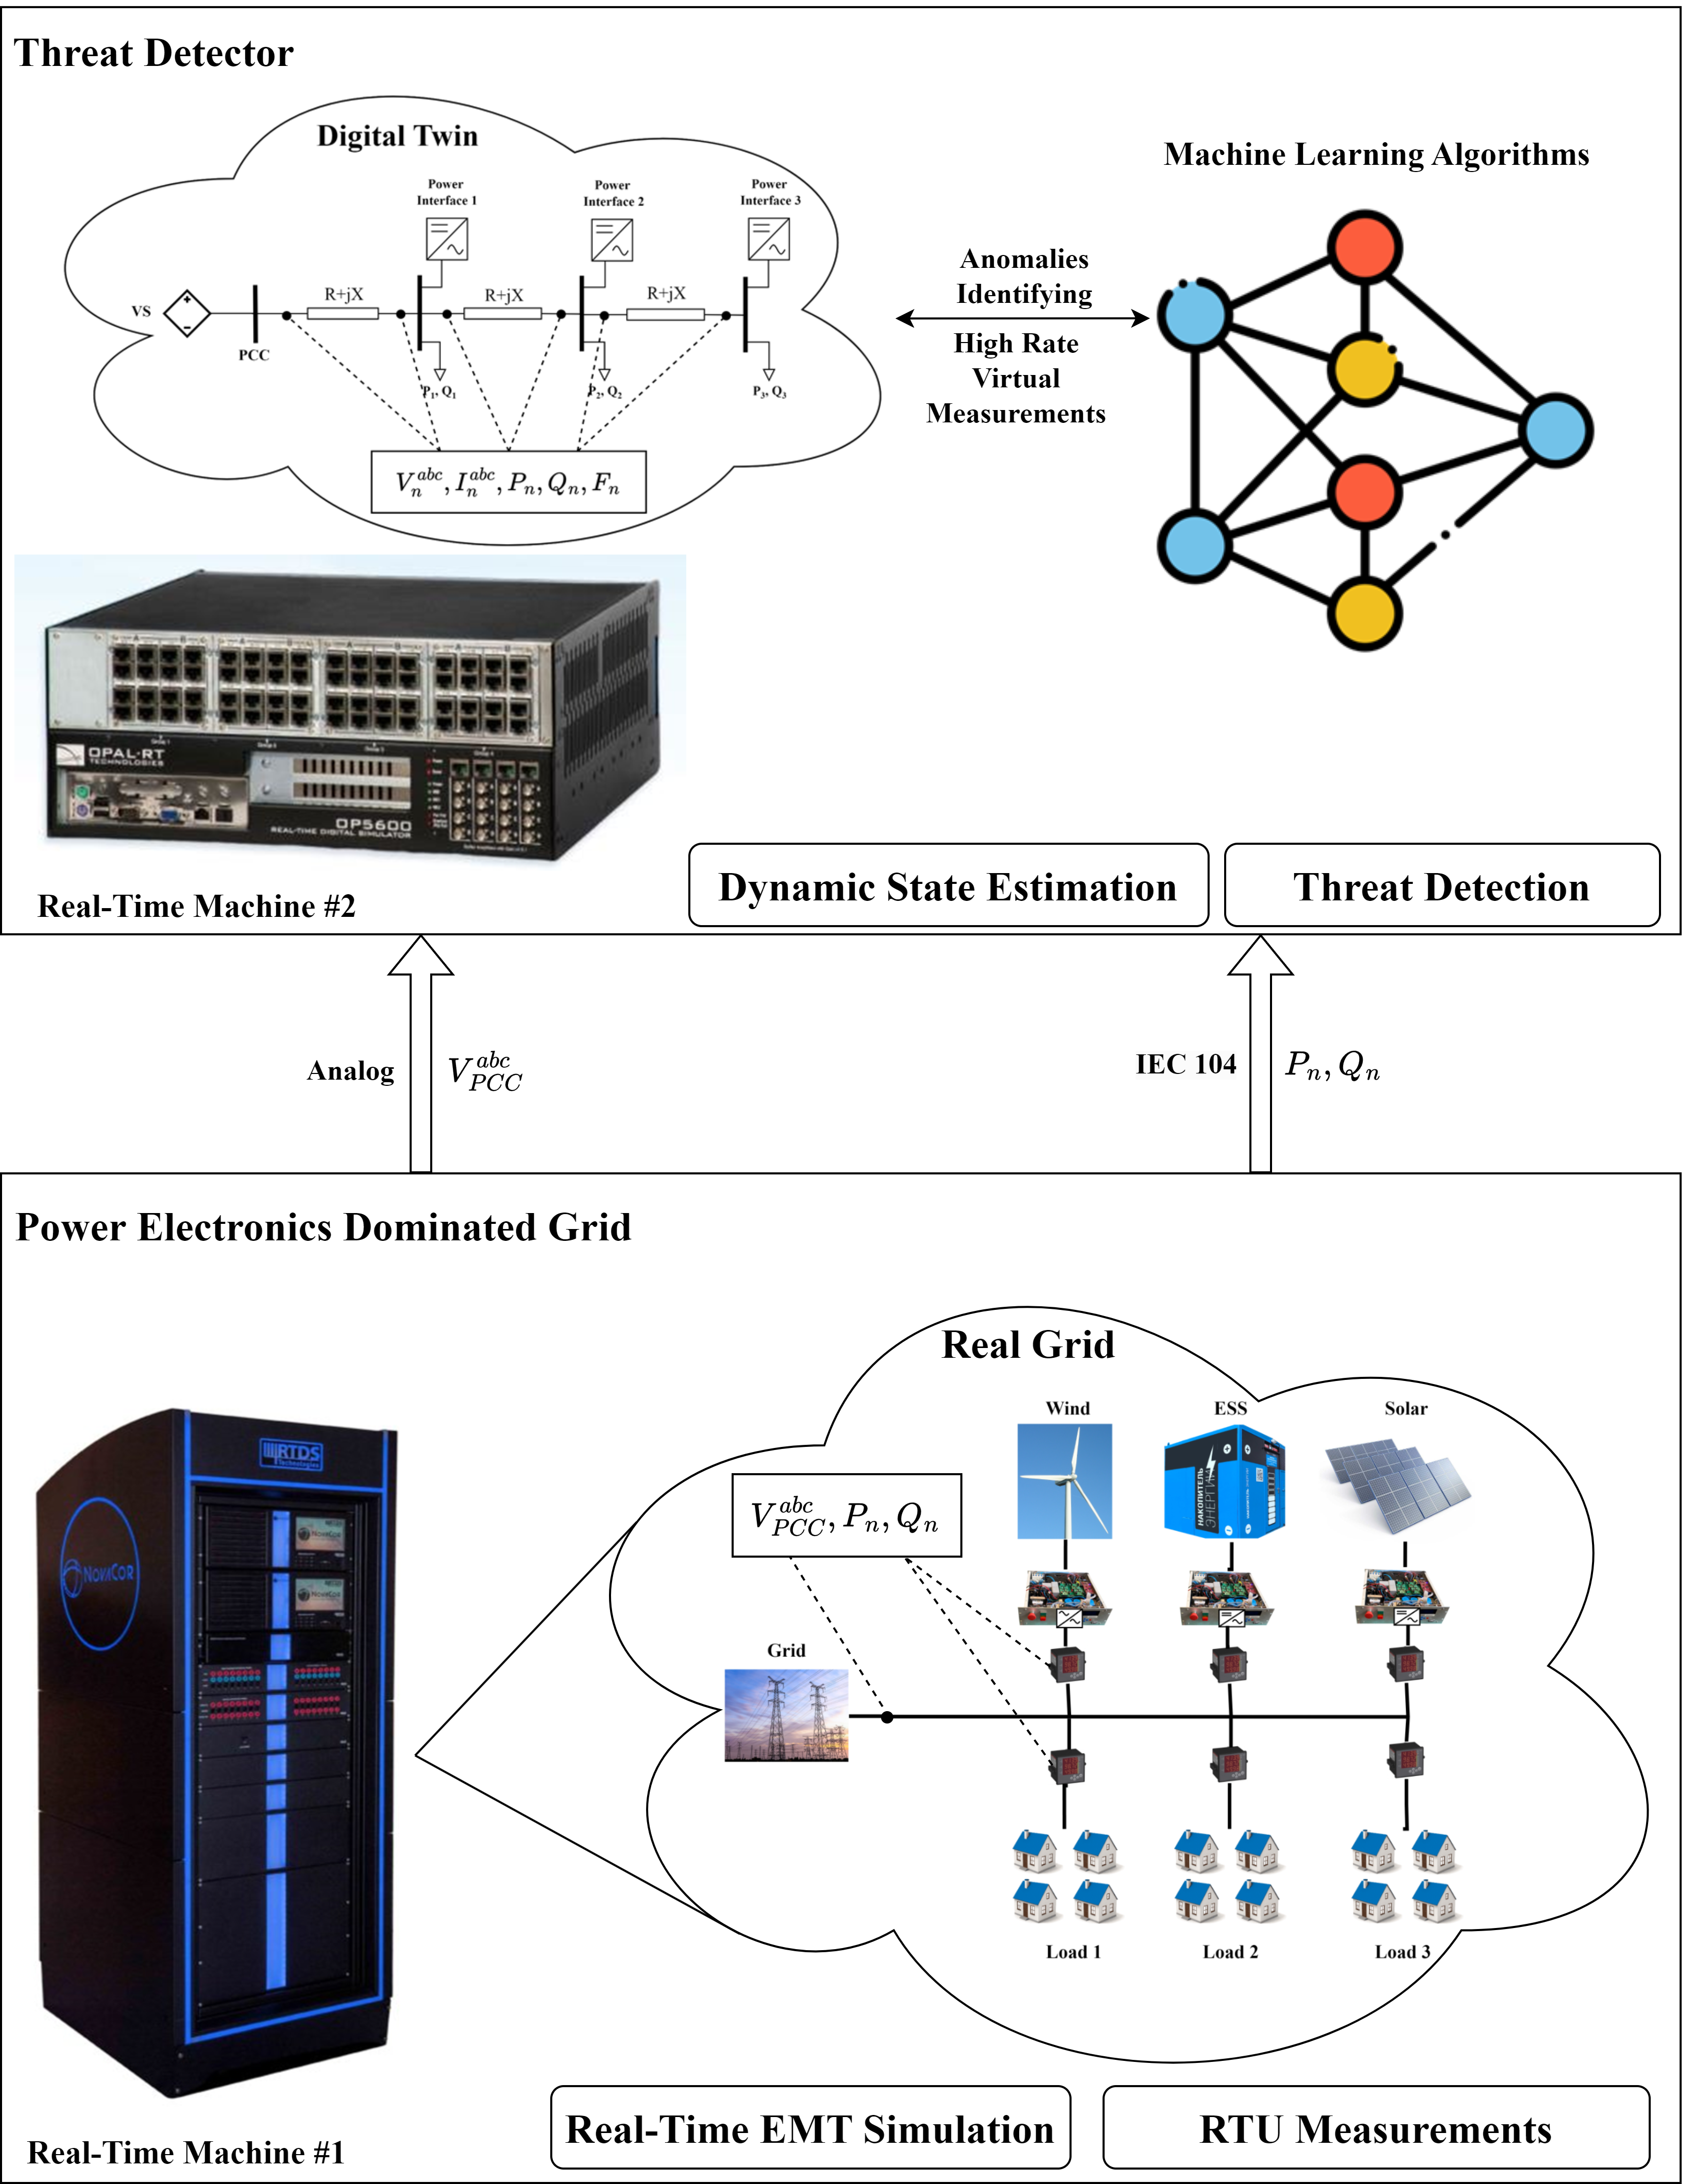
\includegraphics[scale=0.7]{mitm_bench}
    }
    \caption{Test bench system for anomalies detection.}\label{fig:mitm_bench}
\end{figure}

\textbf{Dataset Description}. The datasets utilized in this study comprise time-series measurements collected from a power system and DT under both normal operating conditions and simulated attack scenarios. The data include various electrical parameters, such as:
\begin{itemize}
    \item Power Outputs: Photovoltaic active and reactive power ($P_{pv}, Q_{pv}$), battery active and reactive power ($P_{batt}, Q_{batt}$), wind active and reactive power ($P_{w}, Q_{w}$) and consumer active and reactive powers ($P_{n}, Q_{n}$) – all received from IEDs.
    \item Voltage Levels: Voltage virtual measurements estimation from DT at different nodes within the whole feeder ($V_{1}$ to $V_{6}$).
    \item Frequency virtual measurements estimation from DT at different nodes within the whole feeder ($F_{1}$ to $F_{6}$).
    \item Time Stamps: Temporal markers indicating the time of each measurement.
\end{itemize}

\textbf{ML Setup}. All experiments were conducted under the following conditions. For Random Forest Classifier we set the number of estimators to 100, the maximum depth to 10, the minimum samples split to 10, and the minimum samples leaf to 5. For LSTM Neural Network, we used 32 and 64 hidden Units. The learning rate is adjusted between 0.0001 and 0.001 with a number of epochs between 50 and 150 based on convergence observations. The batch size is selected to optimize training efficiency and convergence stability. A kfold cross-validation was performed with to estimate the model’s generalization capability and to validate its stability across different subsets of data. We applied methods such as dropout and weight decay to prevent overfitting in the neural network. We implemented early stopping based on validation loss to prevent overfitting by halting training when no improvement was observed.

\textbf{Performance Metrics}. To evaluate and compare the models, several performances metrics were employed:
\begin{enumerate}
    \item Accuracy: The ratio of accurately predicted instances to the total number of instances assessed:
    \begin{equation}
        \text { Accuracy }=\frac{T P+T N}{T P+T N+F P+F N},
    \end{equation}
    where $TP$, $TN$, $FP$, and $FN$ represent true positives, true negatives, false positives, and false negatives, respectively.
    \item Precision: The fraction of TPs relative to the total of TPs and FPs, representing the accuracy of positive classifications:
    \begin{equation}
        \text { Precision }=\frac{T P}{T P+F P}.
    \end{equation}
    \item Recall: The proportion of TPs compared to the total of TPs and FNs:
    \begin{equation}
        \text { Recall }=\frac{T P}{T P+F N}.
    \end{equation}
    \item F1-Score: The harmonic mean of precision and recall:
    \begin{equation}
        F 1-\text { Score }=2 \times \frac{\text { Precision } \times \text { Recall }}{\text { Precision }+ \text { Recall }} .
    \end{equation}
    \item Confusion Matrix:A matrix that provides a detailed breakdown of correct and incorrect classifications, allowing for the analysis of the types of errors made by the model.
\end{enumerate}

\textbf{Threat Detection Results}. The performance of both the Random Forest and LSTM models was evaluated under two scenarios: using only data from measurement devices and utilizing the DT-enhanced data. The results of these evaluations are presented in Table \ref{tab:performance_metrics}.

% Requires: \usepackage{multirow}
\begin{table}[h]
    \centering
    \caption{ML Performance Metrics}
    \begin{tabular}{|c|c|c|c|c|}
        \hline
        % \multicolumn{2}{|c|}{TABLE I. ML PERFORMANCE METRICS} \\ \hline
        \multirow{2}{*}{Method} & \multicolumn{4}{c|}{Performance Metrics Without DT} \\ \cline{2-5}
         & Accuracy & Precision & Recall & F1-Score \\ \hline
        Random Forest & 0.7434 & 0.73 & 0.77 & 0.75 \\ \hline
        LSTM & 0.8688 & 0.8325 & 0.8183 & 0.8254 \\ \hline
        \multirow{2}{*}{Method} & \multicolumn{4}{c|}{Performance Metrics With DT} \\ \cline{2-5}
         & Accuracy & Precision & Recall & F1-Score \\ \hline
        Random Forest & 0.8692 & 0.7380 & 0.8748 & 0.8006 \\ \hline
        LSTM & 0.9159 & 0.9417 & 0.8669 & 0.9028 \\ \hline
    \end{tabular}
    
    \label{tab:performance_metrics}
\end{table}

The evaluation of threat detection performance revealed that integrating DT-enhanced data significantly improved the accuracy and overall metrics for both Random Forest and LSTM models.

\section{Computational requirements}\label{sec:ch4/sec6}

To be compatible for real-time execution on both real-time machines and edge devices, the DT is realized as a discrete type Matlab Simulink model with 20 us sampling time. The model is characterized by its state variables, inputs and outputs. As the complexity of the microgrid model increases with the number of loads and IBRs connected to the feeder, the computational time also increases, as shown in Table \ref{tab:comp_req}. A test was carried out for non real-time condition on a working station with one core of Intel i5-1135G7 CPU @ 2.4 GHz processor and 32 GB memory. Notice that the execution time grows significantly fast as the number of states increases, showing a power increase with the power of 1.6 approximately. By extrapolating this relationship to a scenario with 100 devices, we can estimate the execution time to be approximately 220 ms. In industrial scenarios with a substantial number of IBRs, the calculation speed must be significantly increased by utilizing multi-core processing and implementing distributed computation.

\begin{table}[htbp]
\caption{Model Execution Time Characteristic}
\label{tab:comp_req}
\centering
\begin{tblr}{
  hlines,
  vlines,
}
Case  & Loads & IBRs & States & Inputs & Outputs & {Execution Time, ms}          \\
1               & 1     & 1    & 19     & 22     & 46      & 0.14                  \\
2               & 2     & 2    & 37     & 38     & 83      & 0.28                  \\
3               & 3     & 3    & 55     & 54     & 120     & 0.45                  \\
4               & 5     & 5    & 91     & 86     & 194     & 1.1                   \\
5               & 10    & 10   & 181    & 166    & 379     & 3.4                   \\
6               & 20    & 20   & 361    & 326    & 749     & 10                   \\
\end{tblr}
\end{table}

Talking about hard real-time execution, such machines as OPAL-RT allows to run on 1 core the case 5 from  Table \ref{tab:comp_req} with 10 kHz frequency. The extension of the number of devices requires to add additional cores and partitioning of the model in analogy with the MATE concept. The best performance can be reached on the basis of System-On-Chips (SoC) solutions which combines multiple CPU cores with an FPGA. This architecture based on MATE approach described in section \ref{sec:dt_method} allows circuit models to be partitioned and computed in parallel on the CPU cores and the FPGA \autocite{ppmpower_rtbox_compare}. Multiple SoC chips, connected via multi-gigabit optical links, can form a scalable real-time simulation cluster. This enables distributed synchronous computation of large circuit models, such as PEDGs.